% basically this is a template file, you should be able to take it and
% start running.

% the philosophy behind this template is that each chapter or
% chapterlike section goes in a separate file and you use the \include
% command to input it into the final document.  The \includeonly
% command can be used so you only need to work on one or two chapters at a
% time (instead of having to either latex the entire book each time or
% losing cross-references and page numbering)

% copy this file and call it something like mythesis.tex

\documentclass[11pt]{report}
% note that the documentclass can take other option such as
% twoside - for double sided printing
% openright - if double side  chapters always start on odd pages
% openany - if double side chapters start on the next page even or odd
% 12pt can be replaced by 11pt

\usepackage{suthesis-2e}
% options are
% online - now the default
% hardcopy - turns off online includes signature page and copyright page in file 
% engineer - does an engineer thesis instead of a PhD dissertation

%% load other packages you need

%% uncomment the following and create mythesis-macros.sty for all your
%% own macros.  This keeps this top level file looking fairly neat.
% \usepackage{mythesis-macros}

%% certain types of theses require special title page format.  See the
%% style file for the full list.  An example would be that for some of
%% the language departments. 
% \dualthesis \dept{Asian Languages} \languagemajor{Korean} 
%% or education
% \educationthesis

\title{Scaling a Reconfigurable Dataflow Accelerator}
\author{Yaqi Zhang}
%\dept{} % default is Computer Science, uncomment for other departments
\principaladviser{Kunle Olukotun}
% \coprincipaladvisor{}
\firstreader{Subhasish Mitra}
\secondreader{Matei Zaharia}
% \thirdreader{}

%the following command would (if uncommented) allow  only chapter1 and
%chapter2 to be processed
%\includeonly{chapter1,chapter2}

% if you feel real savvy use
% \typein{Now put in includeonly}
% the \typein command stops latex at this point and allows you to type
% in a command such as
% \includeonly{chapter3,chapter5}
% this can save some time and means you don't have to edit this file
% as much.

\usepackage[T1]{fontenc}

%% Font of document
\usepackage{tgpagella}
%\usepackage{tgbonum} %% no good
%\usepackage{bookman} %% no good
%\usepackage{charter} 

\usepackage{graphicx}

\usepackage{listings}           % Code listing
\usepackage{courier}
\definecolor{vbgray}{gray}{0.9}
\definecolor{darkgreen}{RGB} {0, 100, 0}
\definecolor{darkred}{RGB} {255, 0, 0}
\definecolor{orange}{RGB} {255, 128, 0}
\def\tick{{\color{darkgreen} \textbf{\tikz\fill[scale=0.5](0,.35) -- (.25,0) -- (1,.7) -- (.25,.15) -- cycle;}}}
\def\ytick{{\color{orange} \textbf{\tikz\fill[scale=0.5](0,.35) -- (.25,0) -- (1,.7) -- (.25,.15) -- cycle;}}}
\def\x{{\color{darkred} {$\bm{\times}$}}}

\definecolor{red}{RGB}{255,0,0}
\definecolor{vbgray}{gray}{0.9}
\definecolor{darkgreen}{RGB} {0, 100, 0}
\definecolor{darkred}{RGB} {255, 0, 0}
\definecolor{blue}{RGB} {0, 135, 255}
\definecolor{yellow}{RGB} {224, 173, 0}
\definecolor{codegreen}{RGB}{52,123,0}
\definecolor{codegray}{rgb}{0.6,0.5,0.5}
\definecolor{codepurple}{rgb}{0.58,0,0.82}
\definecolor{backcolour}{rgb}{0.95,0.95,0.95}
\definecolor{lightback}{rgb}{0.95,0.95,0.95}
\def\tick{{\color{darkgreen} \textbf{\tikz\fill[scale=0.5](0,.35) -- (.25,0) -- (1,.7) -- (.25,.15) -- cycle;}}}
\def\ytick{{\color{orange} \textbf{\tikz\fill[scale=0.5](0,.35) -- (.25,0) -- (1,.7) -- (.25,.15) -- cycle;}}}
\def\x{{\color{darkred} {$\bm{\times}$}}}

\lstdefinelanguage{Spatial}{
  basicstyle=\fontsize{7}{7}\selectfont\ttfamily,frame=tlbr,framesep=4pt,framerule=0pt,
  tabsize=2,
  basewidth={0.55em, 0.4em},%
  numbers=left,
  showspaces=false,
  keywordstyle=\bfseries,
  breaklines=true,
  columns=fixed,
  %xleftmargin=0.25in,
  firstnumber=auto,
  showstringspaces=false,
  escapechar=@,
  escapeinside={(*@}{@*)},
  morestring=[b]",
  morestring=[b]',
  morecomment=[l]{//},
  morecomment=[s]{/*}{*/},
  backgroundcolor=\color{backcolour},
  commentstyle=\color{codegreen}, %\bfseries,
  numberstyle=\tiny\color{codegray},
  stringstyle=\color{codepurple},
  keywordstyle=[2]\color{blue},
  keywords=[2]{val, def, type},
  keywordstyle=[3]\color{yellow}\bfseries,
  keywords=[3]{Float, Float8, Int, String, T, Void, Bit, Half, FltPt},
  keywordstyle=[4]\color{orange}\bfseries,
  keywords=[4]{Matrix, Array},
  keywordstyle=[5]\color{blue}\bfseries,
  keywords=[5]{StreamIn, StreamOut, DRAM, ArgIn, ArgOut, HostIO, RegFile, Reg, SRAM, SRAM1, SRAM2, FIFO, LIFO, LUT, LineBuffer},
  keywordstyle=[6]\bfseries,
  keywords=[6]{enq, deq, load, store, scatter, gather, :=, push, pop, peek},
  keywordstyle=[7]\color{magenta},
  keywords=[7]{until, par, by, value},
  keywordstyle=[8]\color{red}\bfseries,
  keywords=[8]{C0,C1,C2,C3,C4,C5,C6,C7,C8,C9,C10},
  keywordstyle=\color{magenta}\bfseries,
  morekeywords={Foreach,Reduce,MemReduce,MemFold,Fold,Accel,Stream,FSM,Sequential,if,else,Parallel,Pipe, DummyPipe}
}


\usepackage{booktabs}
\usepackage{multirow}
%\usepackage[numbers,sort&compress]{natbib}
\usepackage{amsmath}
\usepackage{amsfonts}
\usepackage{siunitx}
%\usepackage{minted}

\usepackage[hidelinks]{hyperref}

\usepackage[capitalise]{cleveref}
\usepackage{xspace} 

\newcommand{\name}{SARA\xspace}
\newcommand{\rda}{RDA\xspace}
\newcommand{\rdas}{RDAs\xspace}
\newcommand{\gist}[1]{{\color{blue} #1}}
\newcommand{\todo}[1]{{\color{red} TODO: #1}}

%%
%% Math operators
\DeclareMathOperator*{\argmax}{argmax}
\DeclareMathOperator*{\elmax}{elmax} % Elementwise maximum
\DeclareMathOperator*{\dest}{dest} % Destinations for an operator (its consumers)
\DeclareMathOperator*{\andf}{and}
\DeclareMathOperator*{\maximum}{maximum}

\newcommand{\projb}[1]{\text{proj}_\mathbf{B}(#1)}
\newcommand{\nnint}{\mathbb{Z}_{\ge 0}}
\newcommand{\ind}[1]{\mathbb{1}[#1]}


\begin{document}

% first the preface sections.  

% this includes the file preface.tex which should include the
% following commands
% \beforepreface
% \prefacesection{preface}
% body of the preface

\beforepreface

\prefacesection{Abstract}

%In this talk, I will talk about architectural design and compilation techinques that improves the scaling efficiency of a RDA developed 
%at Stanford--Plasticine.
%Staring with a static-dynamic hybrid network, we show that the hybrid network can improves energy efficiency while providing
%guaranteed success in placement and routing.
%Next, I will talk about compiler techinques that convert applications' complex control hierarchies, such as nested loops and branch conditions, into a streaming dataflow representation that can be efficiently executed by Plasticine with distributed on-chip resources.
%The compiler implements (a) a peer-to-peer (p2p) control paradigm inferred from an imperative programming style that minimizes synchronization overhead, and (b) a mapping strategy that decomposes the computation and memory in a program across a distributed heterogeneous resources.
%By applying these techniques, we show that Plasticine is able to outperform state of art accelerators, such as GPUs and FPGAs, in
%both performance and performance/Watt in various dense, sparse, and streaming applications.

With the slowdown of Moore’s Law, specialized hardware accelerators are gaining tractions 
for delivering 100-1000x performance improvement over general-purpose processors. 
As the performance scaling in multicores is coming to a limit~\cite{multicorescale}, a new
class of accelerators--reconfigurable dataflow architectures (RDAs)--is promising in 
offering high-throughput and energy-efficient acceleration that keeps up with the performance demand.
Instead of dynamically fetching instructions like in traditional processors, RDAs have flexible datapath 
that can be statically configured to spatially parallelize and pipeline the program across
distributed on-chip resources. 
The pipelined execution model and explicitly-managed scratchpad in RDAs eliminate
the performance, area, and energy overhead in dynamic scheduling and conventional memory hierarchy.

To adapt to the compute intensity in modern data-analytic workloads, particularly in the deep learning
domain, RDAs are increasing to a scale that was unprecedented before, compared to the classic coarse-grained
reconfigurable architectures (CGRAs).
With an area footprint of $133\text{mm}^2$ at 28nm, 
Plasticine is a hierarchical RDA with 12.3 TFLOPs of compute power~\cite{plasticine}.
Prior work has shown an up to 76x performance/watt benefit from Plasticine over a Stradix V FPGA 
due to advantage in clock frequency and resource density.
The increase in scale introduces new challenges in on-chip network design to maintain 
the throughput and energy efficiency of RDAs.
Furthermore, targeting and managing RDAs at this scale also require new strategies in mapping, 
memory management, and flexible control to fully utilize the compute power of the accelerator. 

In this work, we focus on two aspects of the software-hardware co-design that impact the usability
and scalability of the Plasticine accelerator. 
One of the biggest challenges that hinders the adoption of these
accelerators is the low-level declarative configuration interface that requires the programmers to
have detailed knowledge about the underlying microarchitecture implementation and hardware
constraints. To address the programmability challenge, we introduce a compiler stack that provides a high-level
programming interface that efficiently translates imperative control constructs to streaming
dataflow execution with minimum synchronization overhead on an on-chip distributed architecture. The
compiler handles the hardware constraints systematically with resource virtualization. To address
the performance challenges, we present a comprehensive study on the on-chip network design for 
reconfigurable dataflow architectures that sustain performance in a scalable fashion with high energy efficiency.

\prefacesection{Acknowledgements}

As a start, I would like to thank the most impactful person in my graduate adventure--my advisor
Kunle Olukotun.
Retrospectively, he provided many constructive suggestions that set forth a good foundation for my research.
While Kunle knows what is right, he allows us to explore and make mistakes.
A frequent question from Kunle during our one-on-ones is ``So, what's the plan?'.
One of the most valuable skills I have acquired from graduate school beyond the technical expertise is the ability to construct an executable plan for a new problem, realize the defects in the initial solution, and persistently refine the implementation, which results in innovations.

Many other Stanford professors have benefited my research from various perspectives.
I would like to thank Subhasish Mitra and Christos Kozyrakis for their past support on the
Plasticine project.
Interactions with Matei Zaharia and Chris R\'e during DAWN retreats also enlarged my scope on 
software advancement in machine learning research and frameworks.
I would also like to thank Juan Rivas to join my defense as my committee chair and evaluating the
contribution of the work for a broader audience.

I have encountered a group of exceptional colleagues at Stanford and
benefited tremendously in my professional skills\footnote{and other random knowledge} during interactions with my peers.
David Koeplinger answered many of my Scala questions and I have learned a great deal about compiler
infrastructures by reading his code.
Raghu Prabhakar had always been extremely helpful and instrumental in research discussions. 
He often put himself in others' shoes that he was always the most popular person on the planet back at school and now at work.
Alex Rucker made a great contribution to Plasticine's network design and introduced a high-level simulator that relieved me from RTL simulation, which undoubtedly expedited my graduation.
Matt Feldman enhanced the Spatial compiler and made it robust, which supported the research of mine and many
others, both inside and outside our group.
Matt also contributed his dog, Daisy, to befriend with everyone and 
provide de-stress after a hard-working Friday afternoon.
Tian Zhao provided generous support on experiment setup and baseline collections during many of my paper deadlines.
I had a great collaboration experience with Matt Vilim, who also introduced me to ergonomic keyboards.
Nathan Zhang contributed considerably to solver-related works and was always the happiest person in the group that positively affected everyone.
Muhammad Shahbaz was particularly helpful on paper editing and helped me identify the impact and contribution of my work.
I had a fun cross-domain collaboration with Rekha Singhal and Jeff Ullman to design new algorithms for our
hardware.

I would also like to thank everyone in Kunle's group and all of the DAWN members, including but not limited to, 
Tushar Swamy, Olivia Hsu, and Luigi Nardi. 
All of you are an important part of my graduate school experience.
I appreciate the hard work our Admins--Dan Moreau and Andrea Brand-Sanchez--had put forth that
offered us a smooth experience for graduate school.

I would like to share my gratitude towards my undergraduate research advisor, Daniel J. Sorin, who has taught the
majority of my architecture classes and inspired my research interests in this area.
I would not have experienced such a fruitful journey and acquainted so many outstanding people
without his mentoring and encouragement.

Last but not least, I would like to thank my friends and family for continuous support during my
graduate school. 
Friends have always been my first source for help ever since I left home and studied abroad.
They have enriched my life beyond research, making the past five years both enjoyable and
unforgettable.
My parents' passion for research has always inspired me to pursue a Ph.D., and their encouragement and
acknowledgments equipped me with tremendous strength and confidence to complete this adventure.
Finally, I would like to thank my boyfriend, Charles, for always by my side during the happiest and the most stressful moments. 
He was especially understanding and supportive that he would
share my household burden during deadlines and accommodate my irregular sleeping and working schedules.
My graduate school journey would be much more challenging and less rewarded without the support from all these people.


%% afterpreface produces a table of contents and any other tables
%% wanted. At the end pagenumbering changes from roman to arabic and
%% is restarted
\afterpreface

\chapter{Introduction (WIP)}

With the end of Dennard Scaling~\cite{dennard}, the amount of performance one can extract from a CPU is reaching a limit.
To provide general-purpose flexibility, CPU spends the majority of energy on overheads, including dynamic-instruction execution, branch prediction, and a cache hierarchy, and less than 20\% of the energy on the actual computation~\cite{mark}.
Even worse, the power wall is limiting the entire multicore family
to reach the doubled performance improvement per generation enabled by technology scaling in the past\cite{multicorescale}.

\chapter{Background (WIP)}

\section{Execution Schedule of Reconfigurable Architectures} 
\begin{figure*}
\begin{subfigure}[b]{0.34\textwidth}
\inputminted{python}{code/spatialeg2.py}
\caption {
}
\end{subfigure}
\hfill
\begin{subfigure}[b]{0.65\textwidth}
\centering
\includegraphics[width=1.0\textwidth]{figs/pipeexec.pdf}
\caption {
}
\end{subfigure}
\caption[Hiearchical pipelining and parallelization on spatial architecture]{
Hierarchical pipelining and parallelization in spatial architecture.
(a) illustrates the runtime and throughput of a hierarchically pipelined and parallelized program on
a reconfigurable spatial architecture. 
At inner level, instructions within each basic
block are fine-grained pipelined across iterations of the inner most loop. 
At outer level, the inner loops are coarse-grained pipelined across the outer loop iterations.
Exploiting multiple levels of pipeline parallelism gives a total throughput of $x+y$ operations per
  cycle, where \emph{x} and \emph{y} are number of operations in the basic blocks.
(b) Vectorizing the inner most loops B and C by \texttt{n} increases the throughput to $(x+y)n$.
(c) Parallelizing the outer loop A by \texttt{m} further increases the throughput to $(x+y)mn$.
}
\label{fig:pipeexec}
\end{figure*}

\begin{figure*}
\centering
\includegraphics[width=0.4\textwidth]{figs/peakutil.pdf}
\caption[Average utilization vs. peak compute density tradeoff]{
 Average utilization vs. peak compute density tradeoff among different architectures.
}
\label{fig:peakutil}
\end{figure*}

\begin{figure*}
\centering
\includegraphics[width=1\textwidth]{figs/perfmodel.pdf}
\caption[High-level performance model of spatial architectures]{
High-level performance model of spatial architectures
}
\label{fig:perfmodel}
\end{figure*}

The key advantage of reconfigurable spatial accelerators, compared to processor-based architectures, 
is the ability to explore multiple levels of pipeline parallelism. 
In traditional Von Neumann architectures~\cite{vonneumann}, like CPUs and GPUs,
a computer consists of a processing unit that performs
computation, a memory unit that stores the program states, and a control unit that tracks execution
states and fetch the instruction to execute. This computing model inherently assumes that
instructions with in a program are executed in-time, maximizing the flexibility to 
context switching between different workloads dynamically.

Reconfigurable accelerators are a direct violation of the von Neumann execution model; 
instructions are statically imbedded in the datapath and executed in-space as supposed to in-time.
One of the disadvantage of reconfigurable hardware is paying the resource cost for infrequently
executed instructions, making it unsuitable for control-heavy workloads that traditional
processors are efficient at.
On the other hand, RDAs are particularly competitive in providing high-throughput, 
low-latency, and energy-efficiency acceleration for these applications.
Data-analytical workloads encompass a wide domains of applications, including image processing,
recognition, machine translation, digital signal processing, network processing, etc.
These applications exhibits a rich amount of data-level parallelism with relatively static control
flow.

\Cref{fig:pipeexec} shows an example of exploiting hierarchical parallization and pipelining on
a spatial architecture, where overall throughput equals to the product of total parallelization factors 
and pipelining depth.
By exploring multiple dimensions of concurrency in the program, spatial architecture is more likely
to achieve a good compute throughput for a wide range of applications.
For applications that are expensive to parallelize due to irregular access patterns, spatial
architectures can increase concurrency on the pipelining dimension.  For application with
embarrassingly parallel workloads, reconfigurable accelerator can 

Another benefit of pipelined execution is easier to achieve good memory performance.
Data accessed by different stage of the pipelines are stored in discrete scratchpads 
instead of a shared cache; improving the effective on-chip bandwidth and capacity.
Using explicitly managed scratchpad also tends to improve locality and 
eliminate cache performance issues, such thrashing.
Across kernels, pipelined execution reduces the amount of off-chip accesses for intermediate
data.
SIMT architectures, like GPUs, relying on high-bandwidth DRAM technology, such has HBM, to sustain
the compute throughput of massively parallelized threads.
While providing over 10x more bandwidth than traditional DDR technologies, HBM is very limited in
capacity, around 16GB as supposed to on the orders of TB for DDR.
As a result, the limited off-chip capacity often restricts the type of applications that
GPUs can support.

%\begin{table*}
  %\centering
%\begin{tabular}{lccc}
  %\toprule
 %Concurrency Level & Instruction & Data & Task/Kernel  \\ \midrule
 %Parallelsim & CPU,\rda & CPU,GPU,\rda & CPU,\rda  \\
 %Pipelining & \rda & \rda & \rda \\
 %\bottomrule
%\end{tabular}
%\caption[Concurrency level explored by different architectures]{
  %Concurrency level explored by different architectures
%}
%\label{tab:conclevel}
%\end{table*}

\section{Plasticine}

\begin{figure*}
\centering
\includegraphics[width=0.8\textwidth]{figs/plasticine.pdf}
\caption[Plasticine chip-level architecture]{Plasticine chip-level architectural diagram}
\label{fig:plasticine}
\end{figure*}

\section{Spatial}

\begin{figure}
\centering
%\newsavebox{\outerProduct}
%\begin{lrbox}{\outerProduct}
\lstinputlisting[language=Spatial,linewidth=0.6\columnwidth]{code/OuterProduct.scala}
%\end{lrbox}
%\begin{tabular}{m{0.01cm} l} & \usebox{\outerProduct}\\ \end{tabular}
  %\inputminted[fontsize=\footnotesize]{scala}{code/OuterProduct.scala}
  \caption{Example of Outer Product in Spatial.}
\label{fig:spatial_app}
\end{figure}

%To target spatial architectures, we use Spatial, an open source domain specific language for reconfigurable accelerators \cite{spatial_koeplinger}.
We use Spatial~\cite{spatial_koeplinger}, an domain specific language for reconfigurable accelerators, 
as the front-end of Plasticine.
Spatial describes applications with nested loops and an explicit memory hierarchy that captures data movement on-chip and off-chip. 
This exposes design parameters that are essential for achieving high performance on spatial architectures, including blocking size, loop unrolling factors, inner-loop pipelining, and coarse-grained pipelining of arbitrarily nested loops. 
To enable loop-level parallelization and pipelining, Spatial automatically banks and buffers intermediate memories between loops. 
An example of outer product---element-wise multiplication of two vectors resulting in a matrix---in Spatial is shown in Figure~\ref{fig:spatial_app}.
%In this example we assume inputs \emph{vecA}, \emph{vecB} and outputs \emph{matC} do not fit on chip.
%First, \emph{C2} and \emph{C4} load tiles of vectors of size \emph{tsA} and \emph{tsB} to on-chip scratchpads \emph{tileA} and \emph{tileB}. 
%Next, loop \emph{C5} computes the outer products and store it to scratchpad \emph{tileC}. 
%Finally, \emph{C6} stores partial results back to DRAM. 
\if 0
Spatial enables inner loop pipelining in \emph{C5} and coarse-grained pipelining between stages of the outer loop (e.g. \emph{C4}, \emph{C5}, and \emph{C6} are pipelined across iterations of \emph{C3}). 
The parallelization factor of the inner most loop (\emph{ip} for \emph{C2}, \emph{C5}, and \emph{C6}) translates to SIMD pipeline and vector network vectorization factor. 
In \emph{C1} and \emph{C2}, \emph{op1} and \emph{op2} are outer loop parallelization factors that allow the programmer to unroll the outer loops and parallelize compute, which can better saturates DRAM bandwidth or balances compute pipelines. 
When scratchpad producers or consumers are parallelized, the scratchpad must be banked to sustain the required bandwidth. 
Scratchpads only contain one level of banking hierarchy. 
Therefore, when more than one dimension of the scratchpad is banked, the high-dimensional banks are mapped across multiple scratchpads. 
In this example, if both \emph{ii} and \emph{jj} (used in the write address of \emph{tileC}) on line 31 are parallelized, \emph{tileC} will be mapped to multiple scratchpads. 
This mapping strategy makes broadcast communication common between producers, banks, and consumers when outer loops are unrolled.
\fi
For spatial architectures, Design Space Exploration (DSE) of parameters
(e.g., \emph{op1}, \emph{op2}, \emph{ip}, \emph{tsA}, \emph{tsB}) is critical to achieve good resource utilization and performance \cite{dse_koeplinger}.



\chapter{Architecture}

In this section, we discuss the architectural advancement on top of the original Plasticine architecture
introduced in~\cite{plasticine}. These architectural additions helps increase the application
coverage or improve the mapping strategies of existing applications by supporting new language
constructs, data types, and improves the utilizations of the hardware. 
Specifically, \Cref{sec:banking_arch} lay outs the datapath changes in order to support more
flexible banking schemes required by general access patterns supported in Spatial; 
\Cref{sec:rnn_arch} discusses the hardware specialization and architectural sizing for machine
learning applications; \Cref{network} provides an extensive study on on-chip network selection 
reconfigurable spatial architectures.

\section{Generic Banknig Support (WIP)} \label{sec:banking_arch}

\section{Plasticine Specialization for RNN Serving} \label{sec:rnn_arch}

Recurrent Neural Networks (RNNs) are a class of sequence models that plays a key role
  in low-latency,
  AI-powered services in datacenters \cite{fowers2018configurable, jouppi2017datacenter}.
In these services,
  the platforms assume that user requests come in individual samples
  and need to be served with very stringent latency window
  for real-time human computer interaction.
  An example of such workload is
  Google Translate, where inference happens concurrently when a user types.
Despite its popularity, RNN model serving is hard to accelerate efficiently.
Modern software and hardware platforms support optimized BLAS routines.

An efficient execution of RNN requires flexibility in supporting more than BLAS kernels, 

Low-precision inference are commonly used to reduce memory footprint of deep learning models and
increase compute density of hardware accelerators.
Plasticine, however, only supports 32-bit operations and datapath.
Using RNN serving as a motivating example, this section discusses the necessary architecture augmentation and
specialization needed to efficiently map real-time inference on Plasticine.

In \Cref{sec:lowprec}, we propose the necessary micro-architectural changes to
  support low-precision arithmetics on Plasticine.
We also discuss architectural parameter selection for Plasticine
  to serve RNN applications efficiently in \Cref{sec:sizing}

\subsection{Mixed-Precision Support} \label{sec:lowprec}
\label{sec:arch:varprec}
Previous works \cite{fowers2018configurable, jouppi2017datacenter}
  have shown that low-precision inference can deliver promising performance
  improvements without sacrificing accuracy.
In the context of reconfigurable architectures such as FPGAs,
  low-precision inference not only increases compute density,
  but also reduces required on-chip capacity for
  storing weights and intermediate data.

To support low-precision arithmetics without sacrificing coarse-grained reconfigurability,
we introduce two low-precision struct types in Spatial: a tuple of 4 8-bit and 2 16-bit floating-point 
numbers, \texttt{4-float8} and \texttt{2-float16} respectively.
Both types packs multiple low-precision values into a single precision storage.
We support only 8 and 16-bit precisions, which are commonly seen in deep learning inference hardwares.
Users can only access values that are 32-bit aligned.
This constraint guarantees that the microarchitectual change is only local to the PCU.
Banking and DRAM access granularity remains intact from the original design.

\begin{figure}
  \centering
  \includegraphics[width=1\columnwidth]{figs/lowprec.pdf}
  \caption{Plasticine PCU SIMD pipeline and low-precision support.
  Red circles are the new operations. Yellow circles are the original opertaions in Plasticine.
  In (d) the first stage is fused $1^{st}, 2^{nd}$ stages, and the second stage is fused
  $3^{nd}$, $4^{th}$ stages of (b).
   }
  \label{fig:lowprec}
  \vspace*{-0.3in}
\end{figure}
Figure \ref{fig:lowprec} (a) shows the original SIMD pipeline in a Plasticine PCU.
Each FU supports both floating-point and fix-point operations.
When mapping applications on Plasticine,
  the inner most loop body is vectorized across the lanes of the
SIMD pipeline, and different operations of the loop body are mapped to different stages.
Each pipeline stage contains a few pipeline registers (PRs)
  that allow propagation of live variables across stages.
%The PRs are accessible as both inputs and outputs of the FU.
%An FU can also read previous stage's PRs
%as its input value.
Special cross-lane connections as shown in red in Figure \ref{fig:lowprec} enable reduction operations.
To support 8-bit element-wise multiplication and 16-bit reduction, we add 4 opcodes to the FU, shown in
Figure \ref{fig:lowprec} (b).
The $1^{st}$ and $3^{rd}$ stages are element-wise, low-precision operations
  that multiply and add 4 8-bit and 2 16-bit values, respectively.
The $2^{nd}$ and $4^{th}$ stages rearrange low-precision values into two registers,
  and then pad them to higher precisions.
The $5^{th}$ stage reduces the two 32-bit value to a single 32-bit value using the existing add operation. 
From here, we can use the original
reduction network shown in Figure \ref{fig:lowprec} (a) to complete the remaining reduction and accumulates
in 32-bit connection.

With 4 lanes and 5 stages,
  a PCU first reads 16 8-bit values,
  performs 8-bit multiplication followed by rearrangement and padding,
  and then produce 16 16-bit values after the second stage.
The intermediate values are stored in 2 PRs per lane.
Next, 16 16-bit values are reduced to 8 16-bit values
  and then rearranged to 8 32-bit value in 2 PRs per lane.
Then, the element-wise addition in 32-bit value
  reduces the two registers in each line into 4 32-bit values.
These values are fed through the
  reduction network that completes the remaining
  reduction and accumulation in two plus one stages.

In a more aggressive specialization,
  we can fuse the multiply and rearange into the same stage.
We also fuse the first low-precision reduction with the next rearange as shown in Figure \ref{fig:lowprec} (d).
In this way, we can perform the entire low-precision map-reduce in 2 stages
  in addition to the original full precision reduction.
In order to maximize hardware reuse,
  we assume that it is possible to construct a full precision FU
  using low-precision FUs.
In addition, we observe that the original reduction network in the SIMD lanes
  could lead to low FU utilization.
To improve FU utilization, we fold the entire tree structure in a single stage.
Figure \ref{fig:lowprec} (c) shows the folded reduction accumulation structure.
Specifically, latter reductions in the tree are mapped to earlier stages in the pipeline.
In this setup, the entire reduction plus accumulation
  is still fully pipelined in $\log_2(\#_{LANE})+1$ cycles
  with no structural hazard.
With fused reduced-precision multiplication and reduction, and folded reduction tree,
  a PCU is able to perform all map-reduce that accumulates $4 \#_{LANE}$
  8-bit values using 4 stages.
All the operations are completed in $2+\log_2(\#_{LANE})+1$ cycles.

\subsection{Sizing Plasticine for RNN Serving} \label{sec:sizing}
Evaluating an RNN cell containing $N$ hidden units and $N$ input features
  requires $2N^2$ computations and $N^2+N$ memory reads.
With large $N$, the compute to memory ratio is 2:1.
The original Plasticine architecture uses a checkerboard layout
  with 1 to 1 ratio between PCU and PMU.
A PCU has 6 stages and 16 lanes, and a PMU has 16 banks.
This provides a 6:1 ratio between
  compute resource and on-chip memory read bandwidth.
As a result of this layout,
  on-chip memory read bandwidth becomes the bottleneck for accelerating RNN serving applications.
Given that RNNs cover a wide range of important applications,
  we select a Plasticine configuration tailored for RNN serving.
Specifically, we choose a 2 to 1 PMU-PCU ratio with 4 stages in each PCU.
Figure \ref{fig:arch} shows the layout of this Plasticine variant.
\begin{figure}
  \centering
  \includegraphics[width=\columnwidth]{figs/arch.pdf}
  \caption{Variant configuration of Plasticine for serving RNN.}
  \label{fig:arch}
  \vspace*{-0.2in}
\end{figure}

\section{On-chip Network}

Achieving scalable performance using spatial architectures while supporting diverse applications requires a flexible, high-bandwidth interconnect.
  %Unfortunately, bandwidth and flexibility are often conflicting goals; static interconnects guarantee bandwidth but lack flexibility due to poor sharing.
  %Dynamic interconnects provide flexibility with better resource sharing but can cause bandwidth bottlenecks due to congestion while requiring more area and power.
 Because modern CGRAs support vector units with wide datapaths, designing an interconnect that balances dynamism, communication granularity, and programmability is a challenging task.

On-chip interconnects can be classified into two broad categories: \emph{static} and \emph{dynamic.}
 {Static interconnects} use switches programmed at compile time to reserve high-bandwidth links between communicating units for the lifetime of the application.
CGRAs traditionally employ static interconnects~\cite{cgraSurvey1, cgraSurvey2}.
In contrast, {dynamic interconnects}, or NoCs, contain routers that allow links to be shared between more than one pair of communicating units.
NoC communication is typically packet-switched, and routers use allocators to fairly share links between multiple competing packets.
Although static networks are fast, they require over-provisioning bandwidth and can be underutilized when a dedicated static link is reserved for a logical link that is not 100\% active. 
While dynamic networks allow link sharing, the area and energy cost to transmit one bit of data is higher for routers than for switches, making bandwidth scaling more expensive in dynamic networks than in static networks.

In this section, we explore the space of spatial architecture interconnect dynamism, granularity, and programmability.
We start by characterizing several benchmarks' communication patterns and showing links' imbalanced
bandwidth requirements, fanout, and data width in \Cref{sec:appchar}. 
Using these insights, we describe a hybrid network with both static and dynamic capabilities to enable both high bandwidth traffic and high resource sharing.
\Cref{sec:network} identifies a space of interconnection networks with static and dynamic capabilities, at multiple granularities. 
Next, We explain our methodology on performance, area, and power modeling in \Cref{sec:net_char}.
Finally, \Cref{sec:net_dse} perform a detailed evaluation of the identified design space for a variety of benchmarks.

Because CGRAs encompass a broad range of architectures, we narrow our study on tile-based CGRAs with
a streaming dataflow execution model, like Plasticine.
At high-level, the architecture may contain a pool of heterogeneous compute and memory tiles (we referring as physical units (PUs)) with a global network.
The network guarantees exactly-once, in-order delivery with variable latency, and communication 
between PUs can have varying granularities (e.g., 512-bit vector or 32-bit scalar).

To generalize the study, we introduce a variant processing engine (PE) style than Plasticine's
pipeline SIMD unit.
The alternative style uses time-scheduled execution, where each PU 
contains a vector function unit (FU) that can execute a small loop of instructions repeatedly in
time.
The scheduling window is small enough that instructions are stored as part of the configuration fabric, 
without dynamic instruction fetch overhead. 
Compared to the pipelined architecture, 
this execution model creates more interleaved pipelining across PUs with communication that is tolerant of lower network throughput, which provides an opportunity to share links.

\subsection{Application Characteristics} \label{sec:appchar}
The requirements of an interconnection network are a function of the communication pattern of the
application, underlying CGRA architecture, and compilation process.
We identify the following key characteristics of spatially mapped applications:

\paragraph{Vectorized communication}
Recent hardware accelerators use large-granularity compute tiles (e.g., vectorized compute units and SIMD pipelines) for
SIMD parallelism~\cite{plasticine, xilinx-acap}, which improves compute density while minimizing control and configuration overhead. 
Coarser-grained computation typically increases the size of communication, but glue logic, reductions, and loops with carried dependencies (i.e., non-parallelizable loops) contribute to scalar communications. 
This variation in communication motivates specialization for the optimal area- and energy-efficiency: separate networks for different communication granularities.

\paragraph{Broadcast and incast communication} 
A key optimization to achieve good performance on spatial reconfigurable accelerators is to explore multiple levels
of parallelization and pipelining, within and across PUs.
By default, pipeline parallelism across PUs introduces high-bandwidth one-to-one communication between dependent stages.
To balance the pipeline throughput, we often need to parallelize the pipeline stage with the most
computation, resulting in one-to-many communication when the receiver stage is parallelized, and
many-to-one communication when the producer stage is parallelized.
When both the producer and the consumer are parallelized, 
the worst case is many-to-many communication, as illustrated in \Cref{sec:memsplit}.
These broadcast and incast patterns introduce challenges in high-performance on-chip networks, as
their bandwidth demands scale quadratically with their chip size in the worst case.

\paragraph{Compute to memory communication}
To encourage better sharing of on-chip memory capacity, many accelerators have shared scratchpads, either distributed throughout the chip or on its periphery~\cite{plasticine, brainwave, streamdataflow}.
Because the compute unit has no local memory to buffer temporary results, the results of all computations are sent to memory through the network.
This differs from the NoCs used in multi-processors, where each core has a local cache to buffer intermediate results.
Studies have shown that for large-scale multiprocessor systems, network latency---not throughput---is the primary performance limiter~\cite{noc}.
For spatial accelerators, however, compute performance is limited by network throughput, and latency is comparatively less important.

\paragraph{Communication-aware compilation}

\begin{figure}
\centering
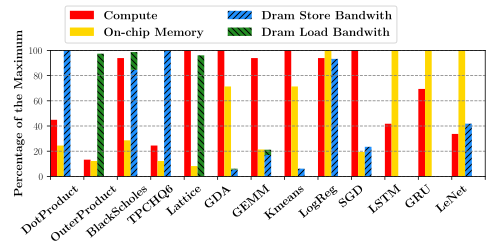
\includegraphics[width=0.8\columnwidth]{network/figs/util_bw2.pdf}
\caption[Resource and bandwidth utilization]{
  Physical resource and bandwidth utilization for various applications.}\label{fig:util_bw}
\centering
\includegraphics[width=0.8\columnwidth]{network/figs/link7.pdf}
  \caption[Application communication patterns]{Application communication patterns on pipelined (a,b) and scheduled (c,d) CGRA architectures.
  (a) and (c) show the activation rate distribution of logical links at runtime. 
  Links sorted by granularity, then rate; darker boxes indicate higher rates.
  The split between green and pink shows the ratio of logical vector to scalar links. (b) and (d) show the distribution of broadcast link fanouts.
 }\label{fig:link}
\end{figure}

\begin{table*}
\centering
  \footnotesize
  \begin{tabular*}{6.25in}{p{0.75in} p{3in} p{2.5in}}
    \bottomrule
    \textbf{Benchmark} & \textbf{Description} & \textbf{Data Size} \\ \midrule
    DotProduct & Inner product & $1048576$ \\ \midrule
    OuterProduct & Outer product &$1024$ \\ \midrule
    BlackScholes & Option pricing &$1048576$ \\ \midrule
    TPCHQ6 & TPC-H query 6 &$1048576$ \\ \midrule
    Lattice & Lattice regression~\cite{garcia2009lattice} &$1048576$\\ \midrule
    GDA & Gaussian discriminant analysis &$127\times1024$ \\ \midrule
    GEMM & General matrix multiply &$256\times256\times256$ \\ \midrule
    Kmeans & K-means clustering &k=64, dim=64, n=8192, iter=2 \\ \midrule
    LogReg & Logistic regression &$8192\times128$, iter=4\\ \midrule
    SGD & Stochastic gradient descent for a single layer neural network &$16384\times64$, epoch=10 \\ \midrule
    LSTM & Long short term memory recurrent neural network &1 layer, 1024 hidden units, 10 time steps \\ \midrule
    GRU & Gated recurrent unit recurrent neural network &1 layer, 1024 hidden units, 10 time steps \\ \midrule
    LeNet & Convolutional neural network for character recognition& 1 image\\ \midrule
  \end{tabular*}
  \caption{Benchmark summary}
  \label{tab:benchmark}
\end{table*}

To study the communication patterns, 
we select a mix of applications from domains where hardware accelerators have shown promising performance and energy-efficiency benefits, such as linear algebra, databases, and machine learning.
Table~\ref{tab:benchmark} lists the applications and their data size.
Figure~\ref{fig:util_bw} shows, for each design, which resource limits performance: compute, on-chip memory, or DRAM bandwidth. 
DotProduct, TPCHQ6, OuterProduct, and BlackScholes are DRAM bandwidth-bound applications. 
These applications use few on-chip resources to achieve maximum performance, resulting in minimal communication.
Lattice (a fast inference model for low-dimensional regression~\cite{garcia2009lattice}), GDA, Kmeans, SGD, and LogReg are compute-intensive applications; for these, maximum performance requires using as much parallelization as possible. 
Finally, LSTM, GRU, and LeNet are applications that are limited by on-chip memory bandwidth or capacity. 
For compute- and memory-intensive applications, high utilization translates to a large interconnection network bandwidth requirement to sustain application throughput. 

Figure~\ref{fig:link}(a,b) shows the communication pattern of applications
characterized on the pipelined CGRA architecture, including the variation in communication granularity. 
Compute and on-chip memory-bound applications show a significant amount of high-bandwidth communication (links with almost 100\% activity). 
A few of these high-bandwidth links also exhibit a high broadcast fanout. 
Therefore, a network architecture must provide sufficient bandwidth and efficient broadcasts to sustain program throughput.
On the contrary, time-scheduled architectures, shown in Figure~\ref{fig:link}(c,d), exhibit
lower bandwidth requirements due to the lower throughput of individual compute PUs. 
Even applications limited by on-chip resources have less than a 30\% firing rate on the busiest logical links; this reveals an opportunity for link sharing without sacrificing performance.

\begin{figure}
\centering
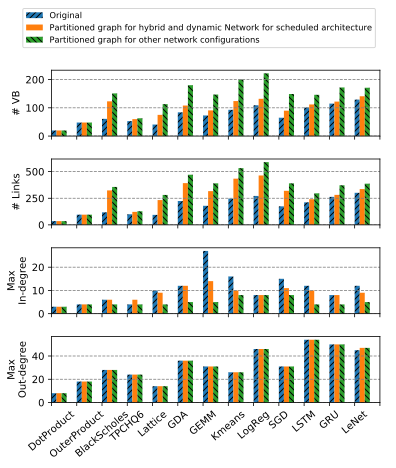
\includegraphics[width=0.9\columnwidth]{network/figs/graph.pdf}
\caption{Characteristics of program graphs.}\label{fig:graph}
\end{figure}

Figure~\ref{fig:graph} shows statistics describing the VU dataflow graph (VGDFG) before and after
the partitioning described in \Cref{sec:resalloc}. 
The blue bars show the number of VUs, number of logical links, and maximum VU input/output degrees in the original parallelized program; the yellow and green bars show the same statistics after partitioning. 
Fewer VUs are partitioned for hybrid networks and dynamic networks with the time-scheduled
architecture.
When a VU in a pipelined CGRA consumes too many inputs or produces too many \emph{distinct} outputs,
\name partitions it to reduce its degree and meet the input/output bandwidth constraints of a purely static network. 
For dynamic and hybrid networks, partitioning is not strictly necessary, but it improves performance
by decreasing congestion at the network ejection port associated with a PU.
We do not partition broadcasts with high output degrees because they are handled natively within the network. 
Finally, the output degree does not change with partitioning because most outputs with a large degree are from broadcast links.

\subsection{Design Space for Network Architectures} \label{sec:network}

We start with several statically allocated network designs, where each SIMD pipeline connects to several switches, and vary flow control strategies and network bisection bandwidth.
In these designs, each switch output connects to exactly one switch input for the duration of the program.
We then explore a dynamic network, which sends program data as packets through an NoC.
The NoC uses a table-based routing scheme at each router to allow for arbitrary routes and tree-based broadcast routing.
Finally, we explore the benefits of specialization by evaluating design points that combine several of these networks to leverage the best features of each.

\subsubsection{Static networks}
We explore static network design points along three axes. 
First, we study the impact of flow-control schemes in static switches. 
In credit-based flow control~\cite{wang2013avoiding}, the source and destination PUs coordinate to ensure that the destination buffer does not overflow.
For this design point, switches only have a single register at each input, and there is no backpressure between switches.
The alternate design point uses a skid-buffered queue with two entries at each switch; using two entries enables per-hop backpressure and accounts for a one-cycle delay in stalling the upstream switch.
At full throughput, the receiver will consume data as it is sent and no queue will ever fill up.

The second axis studied is the bandwidth, and therefore routability, of the static network. 
We vary the number of connections between switches in each direction, which trades off area and energy for bandwidth.
Finally, we explore specializing static links: using a separate scalar network to improve routability at a low cost.

\subsubsection{Dynamic networks}
Our primary alternate design is a dynamic NoC using per-hop virtual channel flow control. 
Routing and Virtual Channel (VC) assignment are table-based: the compiler performs static routing and VC allocation, 
and results are loaded as a part of the routers' configurations at runtime.
The router has a separable, input-first VC and switch allocator with a single iteration and speculative switch allocation~\cite{dallytowles}.
Input buffers are sized just large enough (3 entries) to avoid credit stalls at full throughput.
Broadcasts are handled in the network with duplication occurring at the last router possible to minimize energy and congestion.
To respect the switch allocator's constraints, each router sends broadcasts to output ports sequentially and in a fixed order.
This is because the switch allocator can only grant one output port per input port in every cycle, and the RTL router's allocator does not have sufficient timing slack to add additional functionality.
We also explore different flit widths on the dynamic network, with a smaller bus taking multiple cycles to transmit a packet.

Because CGRA networks are streaming---each PU pushes the result to the next PU(s) without explicit request---the network cannot handle routing schemes that may drop packets; otherwise, application data would be lost.
Because packet ordering corresponds directly to control flow, it is also imperative that all packets arrive in the order they were sent; this further eliminates adaptive or oblivious routing from consideration.
We limit our study of dynamic networks to statically placed and routed source routing due to these architectural constraints.
PUs propagate backpressure signals from their outputs to their inputs, so they must be considered as part of the network graph for deadlock purposes~\cite{hansson2007avoiding}.
Furthermore, each PU has fixed-size input buffers; these are far too small to perform high-throughput, end-to-end credit-based flow control in the dynamic network for the entire program \cite{wang2013avoiding}.
Practically, this means that no two logical paths may be allowed to conflict at \emph{any} point in the network; to meet this guarantee, VC allocation is performed to ensure that all logical paths traversing the same physical link are placed into separate buffers.

\subsubsection{Hybrid networks}
Finally, we explore hybrids between static and dynamic networks that run each network in parallel. 
During static place and route, the highest-bandwidth logical links from the program graph are mapped onto the static network; once the static network is full, further links are mapped to the dynamic network.
By using compiler knowledge to identify the relative importance of links---the link fanout and activation factor---hybrid networks can sustain the throughput requirement of most high-activation links while using the dynamic network for low-activation links.

\subsection{Performance, Area, and Energy Modeling} \label{sec:net_char}

Next section gives a quantitative analysis of the performance, area, and energy trade-offs involved 
in choosing a CGRA network, using benchmarks showing in \Cref{tab:benchmark}.
This section outlines our methodology on how we capture the network performance, area, and energy in our evaluations.
\Cref{tab:notation} gives our notation for various network parameters.

\begin{table}
\footnotesize
  \centering
\begin{tabular*}{0.65\textwidth}{p{1cm} p{8cm}}
  \bottomrule
  \textbf{Notation} & \textbf{Description} \\\midrule
  $[$S,H,D$]$ & Static, hybrid, and dynamic network \\\midrule
  x\# & Static bandwidth on vector network (\#links between switches) \\\midrule
  %$s\#$ & Number of links between switches on static scalar network \\\midrule
  f\# & Flit width of a router or vector width of a switch \\\midrule
  v\# & Number of VC in router \\\midrule
  b\# & Number of buffers per VC in router \\\midrule
  $[$db,cd$]$ & Buffered vs. credit-based flow control in switch \\\midrule
  %$[Scheduled, Pipelined]$ & Time scheduled vs deep pipelined accelerator architectures \\\midrule
\end{tabular*}
\caption{Network design parameter summary.}
\label{tab:notation}
\end{table}

\subsubsection{Simulation}
We use a cycle-accurate simulator to model the pipeline and scheduling delay for the two types of architectures,
 integrated with DRAMSim \cite{dramsim} to model DRAM access latency. For static networks, we model
a distance-based delay for both credit-based and per-hop flow control. 
For dynamic networks, we integrate
our simulator with Booksim \cite{jiang2013detailed}, adding support for arbitrary source routing using look-up tables. 
Finally, to support efficient multi-casting in the dynamic network, we modify Booksim to duplicate broadcast packets at the router where their paths diverge.
At the divergence point, the router sends the same flit to multiple output ports over multiple cycles.
We assume each packet carries a unique ID that is used to look up the output port and next VC in a statically generated routing table, and that the ID is roughly the same size as an address.
When the packet size is greater than the flit size, the transmission of a single packet takes multiple cycles.

\subsubsection{Area and power}
To efficiently evaluate large networks, we start by characterizing the area and power consumption of individual routers and switches
used in various network configurations. 
The total area and energy are then aggregated over all switches and routers in a particular network.
We use router RTL from the Stanford open-source NoC router \cite{becker2012efficient} and our own parameterized switch implementation.
We synthesize using Synopsys Design Compiler with a \SI{28}{nm} technology library and clock-gating enabled, meeting timing at a 1 GHz clock frequency.
Finally, we use Synopsys PrimeTime to back-annotate RTL signal activity to the post-synthesis switch and router designs to estimate gate-level power.

We found that power consumption can be broken into two types: 
inactive power consumed when switches and routers are at zero-load ($P_{\text{inactive}}$, which includes both dynamic and static power),
and active power. The active power, as shown in Section~\ref{sec:net_char}, is proportional to the amount of
data transmitted. 
Because power scales linearly with the amount of data movement, we model the marginal energy to transmit a single flit of data (flit energy, $E_{\text{flit}}$) by dividing active energy by the number flits transmitted in the testbench:
\begin{equation}
  E_{\text{flit}} = \frac{\left(P-P_{\text{inactive}}\right) T_{\text{testbench}}}{\#\text{flit}} 
\end{equation}
While simulating an end-to-end application, we track the number of flits transmitted at each switch and router in the network, as well as the number of switches and routers allocated by place and route. 
We assume unallocated switches and routers are perfectly power-gated and do not consume energy.
The total network energy for an application on a given network ($E_{\text{net}}$) can be computed as:
\begin{equation}
  E_{\text{net}} = \sum_{\text{allocated}} P_{\text{inactive}} T_{\text{sim}}
  + E_{\text{flit}}  \#\text{flit},
\end{equation}
where $P_{\text{inactive}},$ $E_{\text{flit}},$ and $\#\text{flit}$ are tabulated separately for each network resource.

\begin{figure}
\centering
\includegraphics[width=0.8\columnwidth]{network/figs/sweep.pdf}
  \caption{Switch and router power with varying duty cycle.}\label{fig:sweep}
\end{figure}


Figure~\ref{fig:sweep} shows that switch and router power scale linearly with the rate of data transmission, but that there is non-zero power at zero-load. 
For simulation, the duty cycle refers to the amount of offered traffic, not accepted traffic.
Because our router uses a crossbar without speedup \cite{dallytowles}, the testbench saturates the router at 60\% duty cycle when providing uniform random traffic. 
Nonetheless, router power still scales linearly with accepted traffic.

A sweep of different switch and router parameters is shown in Figure~\ref{fig:char}. Subplots (d,e,f) show the energy necessary to transmit a single bit through a switch or router.
Subplot (a) shows the roughly quadratic scaling of switch area with the number of links between adjacent switches.
Vector switches scale worse with increasing bandwidth than scalar switches, mostly due to increased crossbar wire load. 
At the same granularity, a router consumes more energy a switch to transmit a single bit of data, even though the overall router consumes less power (as shown in Figure~\ref{fig:sweep}); 
this is because the switch has a higher throughput than the router.
The vector router has lower per-bit energy relative to the scalar router because it can amortize the cost of allocation logic, whereas the vector switch has higher per-bit energy relative to the scalar switch due to increased capacitance in the large crossbar. 
Increasing the number of VCs or buffer depth per VC also significantly increases router area and energy, but reducing the router flit width can significantly reduce the router area. 

\begin{figure}
\centering
\includegraphics[width=0.8\columnwidth]{network/figs/char.pdf}
  \caption{Area and per-bit energy for (a,d) switches and (b,c,f) routers. 
  The router only has a vector granularity and can be partially clock-gated when sending scalar packets.
  Subplots (f) show the energy of the vector router when used for scalar values (32-bit).}\label{fig:char}
\end{figure}

Overall, these results show that scaling static bandwidth is cheaper than scaling dynamic bandwidth, and a dynamic network with small routers can be used to improve link sharing for low bandwidth communication.  
We also see that a specialized scalar network, built with switches, adds a negligible area compared to and is more energy-efficient than the vector network. 
Therefore, we use a static scalar network with a bandwidth of 4 for the remainder of our evaluation, except when evaluating the pure dynamic network.
The dynamic network is also optimized for the rare instances when the static scalar network is insufficient. 
When routers transmit scalar data, the high bits of data buffers are clock-gated, reducing energy as shown in (f).
Figure~\ref{fig:area} summarizes the area breakdown of all the network configurations that we evaluate.

\begin{figure}
\centering
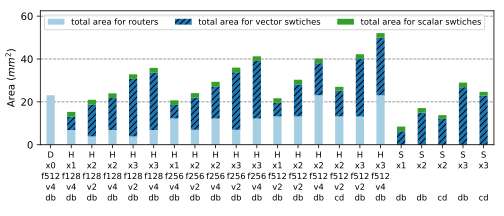
\includegraphics[width=1\columnwidth]{network/figs/area.pdf}
  \caption{Area breakdown for all network configurations.}\label{fig:area}
\end{figure}

\subsection{Network Architecture Evaluation} \label{sec:net_dse}

We evaluate our network configurations in five dimensions: performance (perf), performance per network area (perf/area), performance per network
power (perf/watt), network area efficiency (1/area), and network power efficiency (1/power). 
Among these metrics, performance is the most important: networks only consume a small fraction of the overall accelerator area and energy (roughly 10-20\%). 
Because the two key advantages of hardware accelerators are high throughput and low latency, 
we filter out a network design point if it introduces
more than 10\% performance overhead.
This is calculated by comparing to an ideal network with infinite bandwidth and zero latency.

For metrics that are calculated per application, such as performance, performance/watt, and power efficiency, we first normalize the metric with respect to the 
worst network configuration for that application. 
For each network configuration, we present a geometric mean normalized across all applications. 
For all of our experiments, except Section~\ref{sec:scale}, we use a network
size of $14\times14$ end-point PUs. All vector networks use a vectorization factor of 16 (\SI{512}{bit} messages).

\begin{figure}
\centering
\includegraphics[width=0.8\columnwidth]{network/figs/scale.pdf}
\caption{Performance scaling with increased CGRA grid size for different networks.}\label{fig:scale}
\end{figure}
\subsubsection{Bandwidth scaling with network size}\label{sec:scale}
Figure~\ref{fig:scale} shows how different networks allow several applications to scale to different numbers of PUs.
For IO-bound applications (BlackScholes and TPCHQ6), performance does not scale with additional compute and on-chip memory resources.
However, the performance of compute-bound applications (GEMM and SGD) improves with increased resources, but plateaus at a level that is determined by on-chip network bandwidth. 
This creates a trade-off in accelerator design between highly vectorized compute PUs with a small network---which would be underutilized for non-vectorized problems---and smaller compute PUs with limited performance due to network overhead. 
For more finely grained compute PUs, both more switches and more costly (higher-radix) switches must be employed to meet application requirements.

The scaling of time-scheduled accelerators (bottom row) is much less dramatic than that of deeply pipelined architectures (top row). 
Although communication between PUs in these architectures is less frequent, the scheduled architecture must use additional parallelization to match the throughput of the pipelined architecture; this translates to larger network sizes. 

For pipelined architectures, both hybrid and static networks provide similar scaling with the same static bandwidth:
the additional bandwidth from the dynamic network in hybrid networks does not provide additional scaling. 
This is mostly due to a bandwidth bottleneck between a PU and its router, which prevents the PU from requesting multiple elements per cycle.
Hybrid networks tend to provide better scaling for time-scheduled architectures; multiple streams can be time-multiplexed at each ejection port without losing performance.

\subsubsection{Bandwidth and flow control in switches}

\begin{figure}
  \centering
\includegraphics[width=0.7\textwidth]{network/figs/radar_switch.pdf}
  \caption{
    Impact of bandwidth and flow control strategies in switches.}\label{fig:radar_switch}
\end{figure}

In this section, we study the impact of static network bandwidth and flow control mechanisms (per-hop vs. end-to-end credit-based). 
On the left side of Figure~\ref{fig:radar_switch}, we show that increased static bandwidth results in a linear performance increase and a superlinear increase in area and power. 
As shown in Section~\ref{sec:scale}, any increase in accelerator size must be coupled with increased network bandwidth to effectively scale performance. 
This indicates that network overhead will increase with the size of an accelerator.

The right side of Figure~\ref{fig:radar_switch} shows that, although credit-based flow control reduces the amount of buffering in switches and decreases network area and energy, application performance is significantly impacted. 
This is the result of imbalanced data-flow pipelines in the program: when there are parallel long and short paths over the network, there must be sufficient buffer space on the short path equal to the product of throughput and the difference in latency. 
Because performance is our most important metric, credit-based flow control is not feasible, especially because the impact of bubbles increases with communication distance, and therefore network size.

\subsubsection{VC count and reduced flit width in routers}
\begin{figure}
  \centering
\includegraphics[width=0.7\textwidth]{network/figs/radar_router.pdf}
  \caption{Impact of VC count and flit widths in routers.}\label{fig:radar_router}
\end{figure}
In this experiment, we study the area-energy-performance trade-off between routers with different VC counts. As shown
in Section~\ref{sec:net_char}, using many VCs increases both network area and energy.
However, using too few VCs may force roundabout routing on the dynamic network or result in VC allocation failure when the network is heavily utilized.
Nonetheless, the left side of Figure~\ref{fig:radar_router} shows minimal performance improvement from using more VCs. 

Therefore, for each network design, we use a VC count equal to the maximum number of VCs required to map all applications to that network. 
Figure~\ref{fig:vc} shows that the best hybrid network configurations with 2x and 3x static bandwidth require at most 2 VCs, whereas the pure dynamic network requires 4 VCs to map all applications.
Because dynamic network communication is infrequent, hybrid networks with fewer VCs provide both better energy and area efficiency than networks with more VCs, even though this constrains routing on the dynamic network.

\begin{figure}
\centering
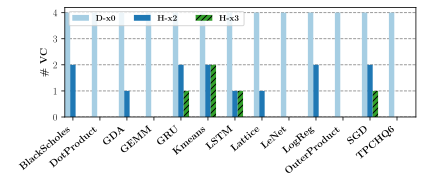
\includegraphics[width=0.75\textwidth]{network/figs/vc.pdf}
  \caption{Number of VCs required for dynamic and hybrid networks. (No VCs indicates that all traffic is mapped to the static network.)}\label{fig:vc}
\end{figure}

We also explore the effects of reducing dynamic network bandwidth by using smaller routers;
as shown in Section~\ref{sec:net_char}, routers with smaller flits have a much smaller area.
Ideally, we could scale static network bandwidth while using a low-bandwidth router to provide an escape path and reduce overall area and energy overhead. 
The right side of Figure~\ref{fig:radar_router} shows that, for a hybrid network, reducing flit width improves area efficiency with minimal performance loss. 

\subsubsection{Static vs. hybrid vs. dynamic networks}

\begin{figure*}
\centering
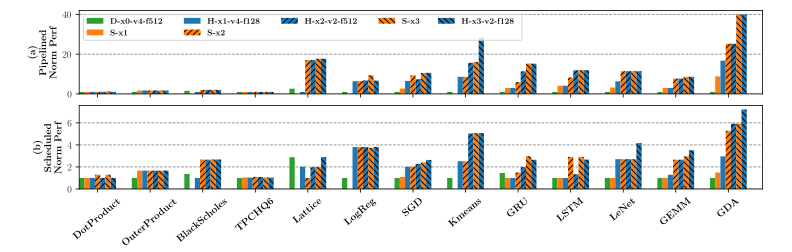
\includegraphics[width=1\linewidth]{network/figs/perf.pdf}
  \caption{Normalized performance for different network configurations.}\label{fig:perf}
\end{figure*}

Figure~\ref{fig:perf} shows the normalized performance for each application running on several network configurations.
For some applications, the bar for S-x1 is missing; this indicates that place and route failed for all unrolling factors.
For DRAM-bound applications, the performance variation between different networks is trivial because only a small fraction of the network is being used. 
In a few cases (Kmeans and GDA), hybrid networks provide better performance due to slightly increased bandwidth.
For compute-bound applications, performance primarily correlates with network bandwidth because more bandwidth permits a higher parallelization factor. 

\begin{figure}
\centering
  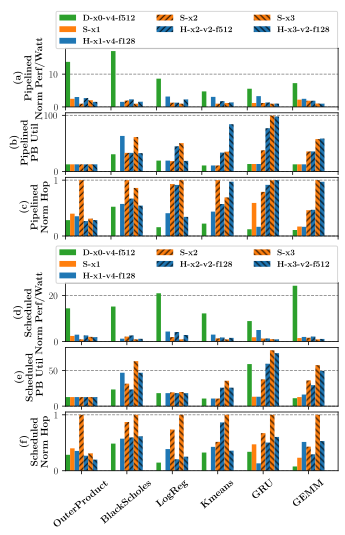
\includegraphics[width=0.9\textwidth]{network/figs/energy.pdf} 
\caption{(a,d): Normalized performance/watt. (b,e): Percentage of compute and memory PUs utilized for each network configuration. 
  (c,f): Total data movement (hop count).}
\label{fig:energy}
\end{figure}

The highest bandwidth static network uses the most PUs, as shown in Figures~\ref{fig:energy}(b,e), because it permits more parallelization. 
It also has more data movement, as shown in (c,f), because PUs can be distributed farther apart. 
Due to bandwidth limitations, low-bandwidth networks perform best with small unrolling factors---they are unable to support the bisection bandwidth of larger program graphs.
This is evident in Figures~\ref{fig:energy}(b,e), where networks D-x0-v4-f512 and S-x2 have small PU utilizations.

With the same static bandwidth, most hybrid networks have better energy efficiency than the corresponding pure static networks, even though routers take more energy than switches to transmit the same amount of data.
This is a result of allowing a small amount of traffic to escape onto the dynamic network: with the dynamic network as a safety net, static PaR tends to converge to better placements with less overall communication.
This can be seen in Figures~\ref{fig:energy}(c,f), where most static networks have larger hop counts than the corresponding hybrid network; hop count is the sum of all runtime link traversals, normalized per-application to the network configuration with the most hops.
Subplots (e,f) show that more PUs are utilized with static networks than hybrid networks.
This is because the compiler imposes less stringent IO constraints on PUs when partitioning for the hybrid network (as explained in Section~\ref{sec:partition}), which results in fewer PUs, less data movement, and greater energy efficiency for hybrid networks.

\begin{figure}
  \centering
\includegraphics[width=0.7\textwidth]{network/figs/radar_best.pdf}
  \caption{Geometric mean improvement for the best network configurations, relative to the worst configuration.}\label{fig:radar_best}
\end{figure}

In Figure~\ref{fig:radar_best}, we summarize the best perf/watt and perf/area (among network configurations with <10\% performance overhead) for pipelined and scheduled CGRA architectures. 
Pure dynamic networks are not shown because they perform poorly due to insufficient bandwidth.
On the pipelined CGRA, the best hybrid network provides a 6.4x performance increase, 2.3x better energy efficiency, and a 6.9x perf/area increase over the worst network configuration. 
The best static network provides 7x better performance, 1.2x better energy efficiency, and 6.3x better perf/area. 
The hybrid network gives the best perf/area and perf/watt, with a small degradation in performance when compared to the static network. 
On the time-scheduled CGRA, both static and hybrid networks have an 8.6x performance improvement. 
The hybrid network gives a higher perf/watt improvement at 2.2x, whereas the static network gives a higher perf/area improvement at 2.6x.
Overall, the hybrid networks deliver better energy efficiency with shorter routing distances by allowing an escape path on the dynamic network.


\chapter{Compiler} \label{sec:compiler}

In this section, we introduce the compiler framework---\name---that targets Plasticine
architecture from high-level programs described in the Spatial language. 

In the following sections, \Cref{sec:control} describes conversion from an imperative paradigm with
a nested control hierarchy to the distributed streaming dataflow execution.
\Cref{sec:resalloc} details program-partitioning passes that decompose program over distributed resources.
\Cref{sec:opt} enumerates several optimizations in \name, and \Cref{sec:par} discuss about PaR and
heuristic generation.

\section{Imperative to Streaming Transformation}
\label{sec:control}

%In a na\"ive approach, we can map each controller in the hierarchy into a VB (\Cref{fig:centralctrl}).
%This strategy suffers from expensive network round-trip delays between the parent and child controllers.
%If the parent controller is an unrolled loop, the parent needs to synchronize with all child controllers, which creates an undesired communication hot spot.
%\Cref{fig:centralctrl}(a) shows an example where synchronization {\em just} between parent and child controllers can produce an incorrect result due to unpredictable network latency.

%The alternative approach explores a different way to execute the expected control schedule correctly. 
%The minimum required synchronization to produce the correct result is to ensure that the computations access the intermediate results in a consistent matter as if the control schedule is strictly enforced. 
%This can be achieved via p2p synchronizations \emph{only} between computations that access a particular shared memory.
%The execution order of computations that access different memories does not need to be enforced, as they do not impact the program outcome.
%Therefore, as long as the computation is executed with the expected number of iterations and the memories are updated consistently, there is no need for any extra synchronization.
%Next, we walk through how \name{} achieves this in more concrete detail.

\subsection{Loop Division (Ready)}
Between the front-end and the back-end abstractions of \name, an obvious gap is that 
the imperative front-end language can contain arbitrarily nested control hierarchy, whereas
the hardware compute engine can only execute operations that are control-free.
To address this issue, we introduce a new type of loop transformation---loop division---for streaming reconfigurable
accelerators.
Similar to loop fission, loop division breaks a single loop into multiple loops.
The difference is that loop fission generates a sequence of sequentially executed loops, whereas
loop division generates loops executing \emph{concurrently}.
Additionally, loop fission materializes the intermediate results across fissioned loops into arrays,
while loop division use queue to communicate across loops.
Each loop generated from loop division can only execute if all of their input queues are not empty.
\Cref{fig:loopexp1} gives an example of a loop fusion vs. loop division.

\begin{figure*}
\centering
\begin{subfigure}[b]{0.28\textwidth}
\inputminted{python}{code/loopexp1.py}
\caption{Input program}
\end{subfigure}
\hfill
\begin{subfigure}[b]{0.31\textwidth}
\inputminted{python}{code/loopexp1fission.py}
\caption{Loop Fission}
\end{subfigure}
\hfill
\begin{subfigure}[b]{0.32\textwidth}
\inputminted{python}{code/loopexp1division.py}
\caption{Loop Division}
\end{subfigure}
\caption[Example of loop fission vs. loop division]{
  (b) and (c) shows the output of loop fission and loop division of the input program (a), respectively.
  In (b), the first loop is executed entirely before executing the second loop. The intermediate
  result \texttt{tmp} is materialized into an array with the same size as the loop range.
  In (b), the two loops can execute concurrently. The intermediate result is materialized into a
  queue. For each iteration, a loop can execute only if all of its queues are non-empty.
  The second loop can execute as soon as \texttt{tmp} receives the first element.
}
\label{fig:loopexp1}
\end{figure*}

When executing loop division on a single-threaded CPU, the CPU must context switching between the
concurrent loops
and executing the one with cleared input dependencies.
Like loop fission, loop division is likely worsening the performance on a processor architecture, as
the worst-case memory footprint of the intermediate result \texttt{tmp} increases from $O(1)$ to $O(N)$.
On RDAs, the divided loops are executing
concurrently in a streaming pipelined fashion. The size of the \texttt{tmp} can be limit to a small fixed
size, efficiently implemented with a hardware FIFO. 
Although loop transformations are generally optimizations on CPUs,
loop division is a required transformation to converts an infeasible program to a feasible one for Plasticine.

Loop fission is not always safe, as it may alter the execution order of the program.
Loop division, on the other hand, does not change the underlying data-dependency and is always safe.
To achieve this, loop division needs to introduce additional dummy data dependencies across divided
loops to enforce the correct execution order.
\Cref{fig:loopexp2} gives an example of an invalid loop fission and a correct loop division.
\Cref{sec:controlalloc} gives more detail on how \name automatically generates the dummy
data-dependencies to preserve program order.

\begin{figure*}
\centering
\begin{subfigure}[b]{0.28\textwidth}
\inputminted{python}{code/loopexp2.py}
\caption{Input program}
\end{subfigure}
\hfill
\begin{subfigure}[b]{0.32\textwidth}
\inputminted{python}{code/loopexp2fission.py}
\caption{Invalid Loop Fission}
\end{subfigure}
\hfill
\begin{subfigure}[b]{0.31\textwidth}
\inputminted{python}{code/loopexp2division.py}
\caption{Loop Division}
\end{subfigure}
\caption[Example of an illegal loop fission and a legal loop division]{
Example of an illegal loop fission and a legal loop division
}
\label{fig:loopexp2}
\end{figure*}

\subsection{Virtual Context Allocation (Ready)} 

\begin{figure*}
\centering
\begin{subfigure}[b]{0.4\textwidth}
\inputminted{python}{code/spatialeg.py}
\caption{Pseudo input example}
\label{fig:contexteg}
\inputminted{python}{code/contextalloc.py}
%\missingfigure[figwidth=1\textwidth]{Spatial IR}
\caption{Initial context allocation}
\end{subfigure}
\hfill
\begin{subfigure}[b]{0.5\textwidth}
\inputminted{python}{code/contextsplit.py}
\caption{Request and response division}
\end{subfigure} \\
\vspace{0.2cm}
\begin{subfigure}[b]{0.23\textwidth}
%\includegraphics[width=1\textwidth]{figs/dep.pdf}
\includegraphics[width=1\textwidth]{figs/ctxdag.pdf}
\caption{Context Graph}
\end{subfigure}
\begin{subfigure}[b]{0.76\textwidth}
\includegraphics[width=1\textwidth]{figs/plasticinetiming.pdf}
\caption{Timing on Plasticine}
\end{subfigure}
\caption[Context allocation and control allocation]{
  Context lowering and control allocation example.
  %Same example as \Cref{fig:spatialegpar} without outer loop
  %unrolling factor equals to 1.
  %(a) has two basic blocks within the inner most controllers \texttt{B} and \texttt{C}.
  \name allocates one context per basic block for \texttt{B} and \texttt{C}, shown in (b). Outer controller \texttt{A} is
  duplicated in both \texttt{ctxB} and \texttt{ctxC}.
  (c) \name separates out a requesting context \texttt{rqstR1} from \texttt{ctxB} for \texttt{R1} 
  and a receiving context \texttt{respW1} from \texttt{ctxC} for \texttt{W1}.
  The resulting dataflow graph is shown in (d). 
  To enforce the forward data-dependency between \texttt{W1} and \texttt{R1}, 
  \name allocates a forward token between \texttt{W1}'s receiving context \texttt{respW1} and
  \texttt{R1}'s requesting context \texttt{rqstR1};
  to enforce the loop-carried WAR dependency between \texttt{R1} and \texttt{W1}, \name allocates a
  backward token \texttt{credit} between \texttt{R1}'s receiving context \texttt{ctxC} and 
  \texttt{W1}'s requesting context \texttt{ctxB}. 
  The backward token is initialized with two elements because \texttt{mem} is double-buffered,
  enabling the writer for two iterations of A before back-pressured.
  %On the writer side, a forward \texttt{token} is a
  %produced and a backward \texttt{credit} is consumed every \texttt{B} iterations; on the reader
  %side, a forward \texttt{token} is consumed and a backward credit is produced every \texttt{C}
  %iterations. 
  For the forward token, the LCA controller between \emph{W1} and \emph{R1} is \emph{A}. The
  immediate child of the LCA controller in ancestor controllers of \emph{W1} is \emph{B}, therefore,
  the enqueue enable of the token is configured to \emph{B.done} in \emph{respW1}. Similarly on the
  receiving cide, the dequeue enable of the token is \emph{C.done} in \emph{rqstR1}.
  The resulting timing of the execution is shown in (e).
}
\label{fig:contextalloc}
\end{figure*}

\begin{figure*}
\centering
\begin{subfigure}[b]{0.5\textwidth}
  \centering
\includegraphics[width=0.6\textwidth]{figs/densespecial.pdf}
\caption{Context dataflow graph}
\includegraphics[width=0.7\textwidth]{figs/denseaddr.pdf}
\caption{Optimization for long address calculation}
\label{fig:densespecial}
\end{subfigure}
\hfill
\begin{subfigure}[b]{0.48\textwidth}
  \centering
\inputminted{python}{code/densectx.py}
\caption{Dense specialization}
\end{subfigure} \\
\vspace{0.2cm}
\begin{subfigure}[b]{1\textwidth}
  \centering
\includegraphics[width=0.85\textwidth]{figs/densetiming.pdf}
\caption{Timing on Plasticine for dense on-chip memory}
\end{subfigure}
\caption[Dense specialization]{
  Specialization for dense memory lowering.
  The same example as \Cref{fig:contextalloc} (a) if the memory is a dense scratchpad.
  (a) and (b) shows the allocated contexts.
  Context \emph{rqstW1} and \emph{rqstR1} are allocated \emph{in the same} VU as the memory. The latency of 
  the forward token and the backward credit take only one cycle, which are not shown in (d).
  The latency to compute read and write addresses are also not shown.
  For complex address calculation, \name split the address computations to separate contexts shown
  in (c). The addresses can be precomputed without waiting for \emph{wdata} for $rqstW1$ and 
  \emph{token} for $rqstR1$.
}
\label{fig:densespecial}
\end{figure*}

At high-level, \name executes the entire program in a pipelined fashion, where each basic block
in the program is a pipeline stage.
As a start, \name allocates a virtual memory to hold each data-structures, and 
a context to execute each basic block within the innermost controllers. 
A basic block maps naturally to a context, as instructions within a basic block are control-free. 
\name makes a copy of all controllers enclosing the basic block in the corresponding context;
these controllers are later converted to counters and control configurations supported by the
hardware. 
Effectively, \name performs loop division such that all basic blocks are perfectly nested.
Contexts are concurrent workers producing and consuming the intermediate data-structures across basic
blocks.

With these controllers, each context can repeatedly execute their basic blocks for an expected number iterations. 
However, data-structures written and read by different contexts are still accessed in random order.
Next, for each virtual memory corresponding to a data-structure, \name examines all contexts accessing the memory,
allocating synchronization tokens across these contexts.
The control token can be viewed as an access grant to the intermediate memory passing between 
the pipelined contexts; the token guarantees the access order of the concurrent contexts is consistent to
the expected order of an imperative program.
The insight is that \emph{as long as all memories are accessed with a program-consistent
order, the final result is identical to a sequentially executed program}.
This way, \name introduces minimum p2p synchronizations among small groups of contexts; contexts
accessing different data-structures are naturally parallelized without impacting the final output.
\Cref{fig:contextalloc} (b) shows an example of the context allocation. 
\Cref{sec:controlalloc} explains how \name allocates the synchronization tokens based on the control
hierarchy of the imperative program.

Unlike traditional out-of-order execution, where both static scheduling in the software and dynamic
scheduling in the hardware search for independent instructions to execute concurrently, 
\name starts with executing \emph{all} basic blocks of a program concurrently,
introducing minimum synchronizations wherever necessary.
Unsurprisingly, a control-heavy program with lots of basic blocks can easily run out of PUs.
Nonetheless, the intended workload for RDAs are data-analytical programs with relatively simple
control flows and abundant data-level parallelism (i.e., most basic blocks having a high repetition
count).
The control flows, however, might not be simple enough that a SIMT architecture, designed for
massive embarrassingly parallel workloads, can still be heavily underutilized.
To map a large program on Plasticine, the program graph must be sliced into multiple chunks.
A single chunk is executed in-space, exploring on-chip parallelism and pipelining;
different chunks are executed in-time by reconfiguring the accelerator.

\subsection{Control Allocation (Ready)} \label{sec:controlalloc}
\label{sec:sync}
\name uses control tokens to enforce the memory access order in an imperative program on a dataflow
architecture. 
In this section, we first explain \emph{how} \name uses tokens to enforce the memory access 
order between distributed contexts and achieves complex control flows on a data-flow architecture;
next, we show \emph{where} \name inserts these tokens and how to minimize inserted tokens while
enforcing the program order.

%This section answers three essential questions for this transformation: 
%\emph{how} to use tokens to enforce the memory access order between two distributed contexts;
%\emph{when} do contexts send the tokens at runtime;
%and \emph{where} do tokens have to be inserted.
%Starting with all contexts execute in parallel, \name introduces \term{control token}s across contexts
%to serialize their execution order based on the program order.
%This control token is no different from a regular data-dependency and can be viewed as 
%an access grant to the shared memory across contexts. 
%By controlling {\em where}, {\em how}, and {\em when} to pass the token, \name is able to maintain a consistent update ordering between the pipelined and parallelized contexts that access the shared memory.

%We refer to a memory access appeared in the input IR as a \emph{declared access}, as supposed to
%memory accesses executed at runtime.
%\texttt{W1} and \texttt{R1} are examples of two declared accesses in \Cref{fig:contexteg}
%In the rest of this section, we will walk through how \name allocates control tokens
%to maintain sequential consistency on Plasticine.

\paragraph{How.} 
The first question is how do we enforce the access order of a memory from two remotely distributed contexts, given the
global network and the memory itself can introduce unpredictable latency.
The memory interface on Plasticine can take a stream of read or write requests, providing a response
packet for each request packet.
Within a single stream, the requests are guaranteed to be served in order. 
Therefore, the read response is a stream of data (not tagged with request address) and the write response is a stream of control tokens without any payload.
To eliminate the round-trip latency, \name divides each memory access in the input IR into a requesting and a receiving context, as shown in \Cref{fig:contextalloc} (c). 
For a read access, \name maps the address generation in a separate requesting context, streaming
addresses to the memory and streaming the data to the receiving context.
Similarly, for a write access, \name allocates a receiving context to accumulate acknowledgments 
for synchronizations.

%We refer to a memory access appeared in the input IR as a \emph{declared access}, as supposed to
%memory accesses executed at runtime.
%\texttt{W1} and \texttt{R1} are examples of two declared accesses in \Cref{fig:contexteg}
To order an access $A$ before an access $B$,
\name allocates a token between the receiving context of access $A$ ($resp_A$) and the requesting context
of access $B$ ($rqst_B$).
This is essential to ensure the memory effect of access $A$ is visible to access $B$, as the memory
might take multiple cycles to serve a request.
For any two accesses enclosed by a loop in the input IR, there could be a loop-carried dependency (LCD) from
the later access in the program order to the earlier access.
When inserting a token for a LCD, the receiver's token buffer is always initialized with at least one token,
enabling the earlier access for the first iteration of the loop. \Cref{fig:contextalloc} (c) shows the
forward and the backward token to enforce two accesses under a loop. The initial element in backward
token breaks the cyclic dependency. 
Borrowing the flow-control
terminology\cite{credit}, we refer to a backward token as a credit.
If the memory is multi-buffered, the credit is initialized with buffer-depth $D$ number of credit, 
enabling the first access to execute $D$ iterations of the enclosed loop before back-pressured.

\name wires up the enqueue/dequeue enable of a token with signals from the duplicated controllers 
in the writer/reader context.
For a token representing the dependency of a queue, the token should be generated/consumed every cycle when the producer/receiver context is active; to achieve this, \name configures the enqueue/dequeue signal
to the \emph{valid} signal of the innermost controller in the requesting/receiving context.
For a token corresponding to a scalar variable or an array, the program expects the producer/consumer
to update/inspect the memory for every iteration of their LCA controller.
\name finds the LCA controller between the writer and the reader contexts of a token,
connecting the \emph{done} signal of LCA's immediate child in the writer/reader context's ancestor controllers to the enqueue/dequeue enable of the token.
\Cref{fig:contextalloc} (c) shows an example of how the enqueue and dequeue signals are configured.

By controlling \emph{when} a token is produced and consumed, \name is able to achieve the complex
and nesting control flows in an imperative program on a dataflow accelerator.
\Cref{sec:datactrl} dives into more complex control constructs with 
data-dependent control flows.

The requesting and receiving contexts pair are general schemes we use on any type of memory with 
multiple cycle access latencies, such as the off-chip DRAM.
In common cases, we can simplify the synchronization logic for certain on-chip memory types.

\subparagraph{Specialization for dense on-chip scratchpad}
Spatial can statically analyze the dense access pattern of on-chip arrays and partitions the memories
to avoid bank conflicts. These memories have a guaranteed single-cycle access latency, 
which simplifies the synchronization.
\name allocates $rqst_A$ and $rqst_B$ contexts \emph{in the same} VB as the accessed memory.
Instead of synchronizing between $resp_A$ and $rqst_B$, \name sends the forward token and the
backward credit between $rqst_A$ and $rqst_B$,
eliminating the need for a receiving context for the write access.
Because memory requests are served in a single cycle, access $A$'s requests would be visible to
access $B$ by the time $rqst_B$ receives the token. Hence, write acknowledgment is no longer needed.
\Cref{fig:densespecial} shows the resulting contexts if \emph{mem} in \Cref{fig:contexteg} is a dense
on-chip array.

\subparagraph{Specialization for non-indexable memory}
For most non-indexable memories like scalar variables and queues in the program, \name directly maps
them to the input buffer of the receiver context if the memory has a single writer and a single
reader.
Non-indexable memory with multiple readers and writers also need synchronization token across
the accessing contexts to enforce a program-consistent accessing order.
%We perform another specialization on non-indexable memories (registers or FIFOs), whose all accesses have no explicit read enables.
%Instead of treating them as shared memories, \name{} duplicates and maps them to local input buffers in all receivers, no longer requiring tokens.
%The sender actor pushes to the network when the token is supposed to be sent, and the receiver dequeues one element from the input buffer when the token is supposed to be consumed.
%This dramatically reduces the synchronization complexity of non-indexable memory in the common case.

\begin{table*}
  \centering
\begin{tabular}{lccc}
  \toprule
 Data structure & Memory type \\ \midrule
  array (fit on-chip) & SRAM \\
  array (not fit on-chip) & DRAM \\
  scalar variable & register \\
  queue & FIFO \\
 \bottomrule
\end{tabular}
\caption[Mapping between data-structure to hardware memories]{
  Mapping between user declared data-structure to underlying hardware memories. 
  Programmers explicitly specify the desired hardware type inside Spatial. 
  In other languages, this table specifies a mapping between software data-structures 
  and hardware memory types on Plasticine.
}
\label{tab:memtype}
\end{table*}

\paragraph{Where.}
\name can serialize every accesses pair of a memory to enforce the program order. However, that
would require $N^2$ tokens for a memory with $N$ accesses ($2N^2$ with LDCs) in the input IR, which can be
unnecessarily expensive.
The second question is how can we minimize the number of inserted token while ensuring a correct execution.
To tackle this problem, \name builds a dependency graph between all accesses of a memory in the input IR; 
the dependency graph is \emph{per data-structure} without unnecessary ordering across different memories.
Next, \name removes edges in the dependency graph, if the removed edge does not relax the ordering
across accesses.
Lastly, for each edge in the reduced dependency graph, \name inserts token between the receiving and
requesting contexts of the source and destination access explained earlier in the \emph{How} section.

\subparagraph{Dependency Graph Construction}
For every access in the IR, \name{} checks on other accesses appeared earlier in the program order
for a possible forward dependency, and later in the program order for a possible loop-carried dependency (LCD). 
%In the example in \Cref{fig:contexteg}, there is a forward data dependency between \texttt{W1} and
%\texttt{R1}, and a write-after-read LCD between \texttt{R1} and \texttt{W1}. 
\name only inserts an edge between two accesses if they potentially interfere, which is a function of
\begin{outline}
  \1 the type of accesses (read vs. write)
  \1 the type of the memory (e.g. SRAM, DRAM)
  \1 and location of the declared accesses in the control hierarchy.
\end{outline}
\Cref{tab:memtype} lists hardware memories available on reconfigurable architectures and software data-structures providing similar program semantics.
The type of the memory matters because they have different programming interface on the hardware.
\Cref{fig:depeg} shows examples of dependency graphs derived from programs.
types.
%For instance, two DRAM read accesses do not interfere because the DRAM interface permits
%multiple concurrent access streams through multiple DAGs\footnote{All DAGs can access the full DRAM
%address space}. 
%%\gist{mension port virtualization}
%Therefore, from the programmer's perspective, users do not need
%to serialize the two contexts reading the same DRAM address. 
%Plasticine's SRAMs, on the other hand, have a single read and write port. 
%Programmers must guarantee that a PMU receives read requests from a single context
%at any point in time for correctness.
%\Cref{tab:interferetab} shows the interference relation between different types of memory across
%accesses.

\begin{table*}
  \centering
\begin{tabular}{lcccc}
  \toprule
  Memory type             & DRAM   & SRAM   & FIFO   & Register \\ \midrule
  read-after-read (RAR)   & \xmark & \cmark & \cmark & \xmark \\
  read-after-write (RAW)  & \cmark & \cmark & \cmark & \cmark \\
  write-after-read (WAR)  & \cmark & \cmark & \cmark & \cmark \\
  write-after-write (WAW) & \cmark & \cmark & \cmark & \cmark \\
 \bottomrule
\end{tabular}
\caption[Interferance Table]{
  Interference table for whether two accesses of the same memory needs to be synchronized by the
  software for each memory type.
}
\label{tab:interferetab}
\end{table*}

\begin{figure*}
\centering
\begin{subfigure}[b]{0.34\textwidth}
\inputminted{python}{code/dep1.py}
\caption {
  Example with outer loop parallelization.
}
\end{subfigure}
\hfill
\begin{subfigure}[b]{0.3\textwidth}
  \centering
\includegraphics[width=0.6\textwidth]{figs/dep1.pdf}
\caption{
  Access dependency graph for \emph{mem} (on-chip) in (a)
}
\end{subfigure}
\hfill
\begin{subfigure}[b]{0.3\textwidth}
  \centering
\includegraphics[width=0.7\textwidth]{figs/dep2.pdf}
\caption{
  Access dependency graph for \emph{mem} (off-chip) in (a)
}
\end{subfigure}
\\
\begin{subfigure}[b]{0.4\textwidth}
\inputminted{python}{code/dep3.py}
\caption{Example with branches}
\end{subfigure}
\begin{subfigure}[b]{0.5\textwidth}
  \centering
\includegraphics[width=0.4\textwidth]{figs/dep3.pdf}
  \caption{Access dependency graph for \emph{mem} (off-chip) in (d)}
\end{subfigure}

\caption[Examples for access dependency graph]{
  Access dependency graphs for example programs. 
  Solid edges indicate forward dependencies and
  dashed edges indicate backward loop-carried dependencies (LCDs).
  In (b) and (c),
  \emph{$W_0$} and \emph{$W_1$} are unrolled accesses for $W$ in lane 0 and 1 of loop \emph{A}
  in (a), respectively.
  (b) is the dependency graph if the memory is mapped to an on-chip memory and (d)
  is the dependency graph if the memory is mapped to an off-chip memory.
  The on-chip version does not need the cross-lane synchronization because 
  lane 0 and 1 are implicitly ordered when \name partitions \emph{mem} 
  (discussed later in \Cref{sec:memsplit}).
  In (d), there is no forward dependency between \emph{W1} and \emph{R0} because the LCA controller of the two accesses is branch \emph{C}, which means the two accesses cannot happen concurrently in
  the same iteration of \emph{A}.
  There is, however, loop-carried dependencies between \emph{R0} and \emph{W1}. 
  Loop-carried
  dependency on the same access (such as between \emph{R0} and itself across iterations of loop \emph{A}) does not need to be enforced as the streaming memory interface preserves ordering
  within a single requesting stream from the same access.
  For each iteration of \emph{A}, \emph{R0} and \emph{W1} will produce and consume a credit from
  each other no matter what value the condition takes. 
  \Cref{sec:datactrl} will elaborate more on branches.
  \emph{R0} and \emph{R1} do not depend on each other because they are both DRAM read accesses.
}
\label{fig:depeg}
\end{figure*}

\subparagraph{Dependency graph reduction}

\begin{figure*}
\centering
\begin{subfigure}[b]{0.34\textwidth}
\inputminted{python}{code/graphred1.py}
\caption {
  Example program with off-chip \emph{mem}
}
\end{subfigure}
\begin{subfigure}[b]{0.3\textwidth}
  \centering
\includegraphics[width=0.6\textwidth]{figs/graphred1.pdf}
\caption{
  Dependency graph before reduction for (a)
}
\end{subfigure}
\begin{subfigure}[b]{0.3\textwidth}
  \centering
\includegraphics[width=0.6\textwidth]{figs/graphred1_after.pdf}
\caption{
  Dependency graph after reduction for (a)
}
\end{subfigure}
\\
\begin{subfigure}[b]{0.34\textwidth}
\inputminted{python}{code/graphred2.py}
\caption{
  Example program with off-chip \emph{mem}
}
\end{subfigure}
\begin{subfigure}[b]{0.3\textwidth}
  \centering
\includegraphics[width=0.6\textwidth]{figs/graphred2.pdf}
\caption{
  Dependency graph before reduction for (d)
}
\end{subfigure}
\begin{subfigure}[b]{0.3\textwidth}
  \centering
\includegraphics[width=0.6\textwidth]{figs/graphred2_after.pdf}
\caption{
  Dependency graph after reduction for (d)
}
\end{subfigure}
\definecolor{pureblue}{rgb}{0, 0, 255}
\caption[Examples for dependency graph reduction]{
  Dependency graphs (b,e) and reduced dependency graph (c,f) of the example programs (a,d).
  Solid edges indicate forward dependencies and
  dashed edges indicate backward loop-carried dependencies (LCDs).
  Colors of the LCD edges indicate the associated loop, \textcolor{pureblue}{blue} for loop \emph{A} and
  \textcolor{red}{red} for loop \emph{B}.
  For the forward edges (black edges), \name uses transitive reduction to remove the redundant
  edges.
  For the backward edge, an edge can be removed if there is still a path from its source to
  destination with all forward edges plus \emph{a single} backward edge with the same loop after the edge is
  removed.
  For example in (c), edge \emph{R2-R1} is removed because there is path \emph{R2-W1-R1}.
  Edge \emph{W2-W1} is removed because there is path \emph{W2-R2-W1}. 
  Edge \emph{R2-W1} cannot be removed because there is no path from \emph{R2} to \emph{W1} with a
  single back edge after the edge is removed.
  \emph{R2-W1} cannot be
  removed in (e) because there is no path from \emph{R2} to \emph{W1} after the edge is removed.
}
\label{fig:graphred}
\end{figure*}

%Enforcing all dependencies in the dependency graph may not be necessary, as enforcing a subset of
%dependencies can be sufficient to enforce the order of the whole graph.
\name reduces the dependency edges in two passes, processing edges for forward and
backward dependencies separately.

For forward dependencies, \name performs a transitive reduction (TR)\cite{tr} on the forward dependency
graph. TR keeps the minimum of edges in a graph that preserves the connectivity of the original
graph, enforcing the same ordering as the original dependency graph.

Next, \name checks if each backward edge can be removed without breaking the execution order between
accesses. 
Each backward edge represents a loop-carried dependency (LCD) and is tagged with the associated loop.
A backward edge can be removed if after removing the edge, there is a path from the source to the
destination node of the edge; the path may contain any forward edges remained from the TR pass,
with \emph{a single} backward edge tagged with the same loop as the removed edge.
\Cref{fig:graphred} shows examples of dependency graph reduction.

The forward edges can be reduced with TR because the forward dependencies
are monotonic, i.e. \emph{A} depends on \emph{B} and \emph{B} depends on \emph{C}
enforces \emph{A} depends \emph{C}. The backward edges are non-monotonic because of the initial
tokens in the destination buffers.

%\begin{figure*}
%\centering
%\includegraphics[width=1.0\textwidth]{figs/synch_mech.pdf}
%\caption{
    %(a) Access dependency graph.
    %(b) Synchronization of two accesses on the same memory.
    %(c) Single-cycle special case.
    %(d) Actors uses local states of controller hierarchy to determine when to send a token.
%}\label{fig:depgraph}\label{fig:token}\label{fig:tokentrick}\label{fig:tokenwhen}
%\end{figure*}
%%\ms{repeated caption, rather give a single caption.}


\subsection{Data-Dependent Control Flow (Ready)} \label{sec:datactrl}
Using the synchronization discussed in \Cref{sec:sync}, \name can support control constructs that 
typically are not supported on dataflow accelerators, such as branches and while loops.
Most dataflow accelerators do not support control divergence. SIMT architectures, like GPUs,
implement branches with predications and pay the latency penalty of both branch cases.
To enable these flexible control, the control path of the architecture must permit data dependencies.
\Cref{fig:controlarch} details the required changes in the control path to support these features.

\paragraph{Dynamic Loop Range}
\Cref{fig:dynrange} shows an example of loops with data-dependent ranges. 
\name uses a context to compute the loop bounds, which are treated as input dependency to the context 
that maps the loop body.
\begin{figure*}
\centering
\begin{subfigure}[b]{0.4\textwidth}
\inputminted{python}{code/dynrange.py}
\caption{Input program}
\end{subfigure}
\hfill
\begin{subfigure}[b]{0.5\textwidth}
\inputminted{python}{code/dynrangectx.py}
\caption{Context data-flow graph}
\end{subfigure}
\caption[Example of dynamic loop range]{
  (a) shows an example program with dynamic loop range. 
  Expressions to generate the loop bounds belongs to a basic block that gets mapped to \texttt{ctx1}.
  \name maps the loop bound as a data-dependnecy to context that maps the inner loop context, and
  configures dequeue signal of \texttt{bound} stream to counter \texttt{B.done}.
}
\label{fig:dynrange}
\end{figure*}

\begin{figure*}
\centering
  \vspace{-1cm}
\begin{subfigure}[b]{0.45\textwidth}
\inputminted{python}{code/branch.py}
\caption{Input program}
  \vspace{0.2cm}
\includegraphics[width=0.8\textwidth]{figs/branchctx.pdf}
\caption{Dataflow graph}
\end{subfigure}
\hfill
\begin{subfigure}[b]{0.48\textwidth}
\inputminted{python}{code/branchctx.py}
\caption{Context configuration}
\end{subfigure}
\\
  \vspace{0.2cm}
\begin{subfigure}[b]{\textwidth}
  \centering
\includegraphics[width=0.8\textwidth]{figs/branchtiming.pdf}
\caption{Timing}
\end{subfigure}
\caption[Branching example]{
  An example program with a branch. 
  (d) shows the timing of execution with $A=4$, $D=3$, and $F=2$.
}
\label{fig:branch} 
\end{figure*}

\paragraph{Branch Condition}
\name supports both predictions and branches with control divergence.
Branches within the innermost loops are implemented with predications such that the loop can still be
vectorized across SIMD lanes.
This is very similar to a SIMT architecture, where all lanes execute the \emph{if} clause followed by the \emph{else} clause, masking off the memory access for the disabled lanes.
The total number of SIMD stages required is the total operations in both the \emph{if} and the \emph{else} clauses.

For a branch in an outer loop,
the branch condition is treated as a data-dependent enable signal for controllers under the branch clauses.
If the controller is disabled, its \emph{done} signal raises to high immediately.
Output tokens depending on the {\em done} signal will be immediately sent out.
This way, the controller under a branch condition does not need to execute if the outer branch
evaluates to false.

\Cref{fig:branch} shows an example with a branch statement.
The input program in (a) writes and reads the memory \emph{mem} on even and odd cycles of
the outer loop \emph{A}, respectively. 
\name maps the three basic blocks in the program in three
contexts, \emph{ctxB}, \emph{ctxD}, and \emph{ctxF}, as shown in (b) and (c). 
For the read and write accesses, \name
allocates a context \emph{respW} to accumulate write acknowledgments and a context \emph{rqstR} 
to generate read requests. 
\emph{ctxB} generates the branch conditions for both the \emph{if} and the \emph{else} clauses.
The conditions are sent as data dependencies to contexts mapping the basic blocks under the branch conditions.

\Cref{fig:branch} (d) shows the timing of execution.
As \emph{ctxB} has no dependencies, \emph{ctxB} computes the conditions for all iterations of
\emph{A} in
pipelined fashion and broadcasts the conditions to the receiver contexts.
The \emph{if} contexts (\emph{ctxD}+\emph{rspdW}) receives a \texttt{true} condition for the first
iteration of \emph{A} ($A_0$), 
executing all iterations of D, and passes a token to the \emph{else} (\emph{rqstR}+\emph{ctxF}) contexts.
Because \emph{mem} is double-buffered, the credit is initialized with two elements in the
receiver's input buffer, enabling the \emph{if} contexts to execute two iterations of outer loop
\emph{A} before
waiting for the \emph{else} contexts. For the second iteration of loop \emph{A} ($A_1$), the \emph{if} contexts
receives a \texttt{false} condition for branch \emph{C}.
Therefore, the enclosing loop controller \emph{D}'s \emph{done} signal is immediately high, sending the
token to \emph{rqstR} context right away.
On the other side, the $A_0$ of the \emph{else} contexts is blocked by the token from
the \emph{if} contexts. 
As soon as the token arrives, the \emph{else} contexts send out the credit immediately,
Next, the \emph{else} contexts check for the second token, 
and executes loop \emph{F} for $A_1$.

Both the \emph{if} and the \emph{else} contexts only execute if their enclosed branch clauses are
evaluated to be true. More interestingly, \Cref{fig:branch} (d) shows a overlapping execution of the
\emph{if} and \emph{else} clauses across iterations of A. 
The hardware for both \emph{if} and \emph{else} clauses are active almost all time.
If the latency of loop \emph{D} and \emph{F} are both $L$, 
the total runtime for $N$ iterations of loop \emph{A} would be on the order of $\frac{N}{2}L+L$
on Plasticine, assuming L and N are large.
\emph{This is almost twice as fast as a traditional coarse-grained pipelining with hierarchical FMS
schedulers}, like Spatial's FPGA back-end, whose runtime is $NL+L$.

\paragraph{Do While Loops}

\begin{figure*}
\centering
  \vspace{-1cm}
\begin{subfigure}[b]{0.45\textwidth}
\inputminted{python}{code/dowhile.py}
\caption{Input program}
  \vspace{0.2cm}
\includegraphics[width=0.8\textwidth]{figs/dowhile.pdf}
\caption{Dataflow graph}
\end{subfigure}
\hfill
\begin{subfigure}[b]{0.48\textwidth}
\inputminted{python}{code/dowhilectx.py}
\caption{Context configuration}
\end{subfigure}
\\
  \vspace{0.2cm}
\begin{subfigure}[b]{\textwidth}
  \centering
\includegraphics[width=0.6\textwidth]{figs/dowhiletiming.pdf}
\caption{Timing}
\end{subfigure}
\caption[Do while example]{
  An example program for do while loop. 
  Loop \emph{A} in (a) is a loop running forever, with a conditional \emph{stop} variable.
  The break statements in (c) corresponds to configuring the stop signal of the enclosing controller \emph{A}
  to the output of the stop input buffer. The stop buffer is dequeued every cycle controller \emph{A} is active.
}
\label{fig:dowhile} 
\end{figure*}

The \emph{do while} construct is very useful to express iterative convergence algorithms or handle external
data stream with a last-bit signal that terminates the execution.
A \emph{do while} loop works very similarly to a loop with dynamic range, except the loop has a very long
initialization interval. The earliest starting time for the second iteration of the loop is when the while condition is resolved.
The while condition is a data-dependency to all contexts mapping the basic blocks enclosed by the while loop.
%This while condition is a loop carried dependency, assuming the first value is produced after the first
%iteration.
There is a loop-carried dependency between the producer of the condition within the while loop body
and the loop controller that consumes a value of condition every iteration.
\Cref{fig:dowhile} shows an example with a do-while loop.

%The break statement in (a) translates to a \emph{stop} register associated with the controller of loop
%\emph{A}. 
Loop \emph{A} reads and block \emph{C} writes a value of stop for every iteration of loop
\emph{A}.
\Cref{fig:dowhile} (b) shows the dataflow graph, mapping each basic block to a context.
\emph{ctxC} computes the stop condition, which is used by both \emph{ctxC} and \emph{ctxB}.
There is a loop-carried dependency between the reader of \emph{stop} from loop \emph{A} and the
writer of stop from block \emph{C}. Therefore, the stop streams in (c) are initialized with 
\texttt{False} to enable the execution of the first iteration.
The \emph{accum} variable in (a) has two readers in block \emph{B} and block \emph{D}; one has a
loop-carried dependency with the writer (line 9) and the other has a forward data-dependency (line
11). 
Therefore, the variable is mapped to two copies of \emph{accum}, one for each reader. 
Because the accumulate operation is a single operation ADD, the accumulator gets optimized to the special
accumulate pipeline register \emph{accum1}, 
Without this optimization, \emph{accum1} would be another \texttt{ScalarStream} with an initial
element 0.
The other \emph{accum} becomes a scalar stream \emph{accum2}, written by \emph{ctxB} when loop \emph{A}
is done.
(d) shows the timing of execution. As we can see, the initialization interval across iterations of
A in the steady-state is bounded by the latency to evaluate \emph{stop}, which is the number of
operations in stop expression rounded up to a multiple of 6 stages because the data must
propagate to the end of each SIMD pipeline.

\paragraph{Procedure Calls}
Our front-end language Spatial currently does not capture procedure calls; 
all functions are inlined in the IR and do not share resources. 
In future work, we can extend \name's token mechanism to handle the procedure call easily. 
The reused hardware corresponding for a function call 
can be viewed as a shared resource like memories; contexts with callers and callees of the procedure call
must pass tokens to serialize their access order.

\subsection{Virtual Unit Allocation (Ready)}
After all contexts and shared memory are allocated and synchronized, 
\name moves each floating context into a VU, which later maps to a PU.
In the resource allocation phase, \name might partition the big contexts into multiple VUs, and small contexts into a single VU. 
Contexts created with dense specialization mentioned earlier must stay in the same VU as their
memory during partitioning.
When contexts are merged into a single VU, they are still
separate contexts triggered independently.

\section{Resource Allocation} \label{sec:decompose}

The output of the transformation (\Cref{sec:control}) is a VUDFG that 
can execute on a Plasticine with infinite-sized physical units (PUs).
The \emph{Resource Allocation} phase enforces and addresses constraint violations given 
the specification of the Plasticine units. 
At the end of this phase, \name assigns each VU in the VUDFG graph to a PU type with required
resources; the placer then takes the type assignments and determines the final placement.

Accelerators often have heterogeneity in compute resources to improve efficiency for commonly used
special operations.
In Plasticine, PMUs and DAGs have specialized compute pipelines for address calculation that are 
less capable than the compute pipeline in PCUs.
However, heterogeneity tends to reduce average utilization because different applications, and even the same
application with different data sizes, can vary highly in the desired ratio among different resource.
A compute-bound application, for example, can heavily underutilize the DAGs and PMUs.
To address this problem, \name model the virtual to physical assignment as a constraint satisfaction problem; 
each VU consumes a set of resources and can only be assigned to a PU if the PU processes the required resources. 
%Instead of using heuristics to assign certain a type of VU to a type of PU, we
\Cref{tab:resource} shows the types of resources in Plasticine's heterogeneous units.
For example, special connection to off-chip memory interface is
also treated as a type of resource in the DAG, which forces virtual contexts accessing DRAM to map to DAGs. 
On the other side, regular contexts with non-vectorized fixed-point operations can also be mapped to spare DAGs.
\begin{table*}
  \centering
\begin{tabular}{lcccc}
  \toprule
  Feature & PCU & PMU & DAG & Host Unit\\ \midrule
  Vector lane width & 16 & 16 & 1 & 1 \\
  Fixed-point op & \cmark & \cmark & \cmark & \xmark\\
  Float-point op & \cmark & \xmark & \xmark & \xmark\\
  Reduction tree & \cmark & \xmark & \xmark & \xmark\\
  \# Vector FIFO & 6 & 6 & 4 & 0\\
  \# Scalar FIFO & 6 & 6 & 4 & 16\\
  \# Control FIFO & 16 & 16 & 4 & 16\\
  Scratchpad banks & 0 & 16 & 0 & 0 \\
  Scratchpad capacity & 0 & 256kB & 0 & 0\\
  MergeBuffer & \cmark & \xmark & \xmark & \xmark\\
  Splitter & \cmark & \xmark & \xmark & \xmark\\
  Scanner & \cmark & \xmark & \xmark & \xmark\\
  Access to DRAM Interface & \xmark & \xmark & \cmark & \xmark \\
  Access to Host IO & \xmark & \xmark & \xmark & \cmark \\
 \bottomrule
\end{tabular}
\caption[Mapping between data-structure to hardware memories]{
  MergeBuffer, Splitter, and Scanner are new hardware introduced in \cite{gorgon} and \cite{capstan}
  to support database and sparsity in Plasticine.
}
\label{tab:resource}
\end{table*}

\begin{algorithm}
  \Fn(\tcc*[h]{A recursive pruning function}){prune(G, pruners)}{
    \KwData{G: bipartite graph between VUs and PUs}
    \KwData{pruners: a list of constraint pruners to check
    and fixes constraint violations}
    \KwResult{The function update G by removing VU-PU edges that violates constraints guarded by
    pruners. The function may fail and raise an exception.}

    \For{pruner \KwTo pruners}{
      \For{v \KwTo G.keys()}{
        \For{p \KwTo G[v]} {
          \If{!pruner.fit(v,p)} {
            G[v] -= p\;
          }
        }
        \If{G[v].empty()} {
          \tcc{Partition VU v based on resource constraints registered in pruner. 
          Not all resources can be partitioned and this step may fail.
          If succeeded, the function returns a new set of VUs.}
          V' = pruner.partition(v)\;
          G' = \KwNew BipartiteGraph()\;
          G'[V'] = G.values()\;
          prune(G',pruners)\;
          G -= v\;
          G[V'] = G'[V']\;
        }
      }
    }
  }
  \vspace{0.5cm}
  \Fn(\tcc*[h]{Allocation Algorithm}){alloc(V, P, pruners)}{
    \KwData{V: a set of VUs from the VUDFG}
    \KwData{P: a set of PUs on the hardware}
    \KwData{pruners: a list of constraint pruners to check
    and fixes constraint violations}
    \tcc{Initialize a complete bipartite graph}
    G = \KwNew BipartiteGraph()\;
    G[V] = P\;
    \tcc{Constraint resolution}
    prune(G, pruners)\;
    \tcc{Global merging}
    merge(G)\;
    \tcc{Virtual to physical assignment}
    backtracking\_assign(G)\;
  }
  \caption{Resource allocation}
  \label{algo:resalloc}
\end{algorithm}
 
%% backtracking_assignment(vu, dom)
As shown in \Cref{algo:resalloc}, the \emph{resource allocation} phase contains three steps:
\emph{constraint resolution}, \emph{global optimization}, and \emph{virtual to physical assignment}.
\name uses a VU-PU bipartite graph (\texttt{G}) to keep track of potential valid assignments between the two.
Initially, \texttt{G} is initialized to a complete bipartite graph, i.e. all VUs can be assigned to
all PUs.

\paragraph{Constraint Resolution}
A list of constraint pruners, each considering a set of on-chip resources, 
incrementally remove the VU-PU edges that violate the resource constraints.
If a VU \texttt{v} has no mappable PU after pruning, the pruner attempts to fix the violation by
decomposing the VU into multiple VUs. 
Not all resources can be composed and the partitioning transformation may fail.
If succeeded, the partitioner generates a new set of VUs \texttt{V'}. \name starts a new complete bipartite
graph between \texttt{V'} and all resources \texttt{P}, and recursively prune on \texttt{V'}.
If succeeded, the original graph \texttt{G} is updated with \texttt{V'} and their pruned resources.

\paragraph{Global Merging}
After all VUs have at least one PU in the bipartite graph, \name triggers a global optimization that merges 
small VUs into a larger VU to reduce fragmentation in allocation.
Each type of resource has a summation rule to compute how the resource usage change if two VUs are merged
together.

\paragraph{Virtual to Physical Assignment}
Next, \name performs a quick heuristic check on the bipartite graph to see if there exists a possible assignment with enough PUs, and provide feedback on the critical resources, otherwise.
Finally, \name assigns each VU to a PU type with a backtracking search on the pruned bipartite
graph.

This approach can be easily extended to handle new heterogeneous tile in the hardware by registering
new resources and partitioning rules.
The rest of this section will focus on two types of partitioning transformations---memory and
compute partitioning in \Cref{sec:memsplit} and \Cref{sec:compsplit}. 
%We have another partitioner encoding valid rule to decompose a BlackBox IP block available on the RDA.

\subsection{Memory Partitioning} \label{sec:memsplit}
The memory pruner addresses VUs with virtual on-chip scratchpad memories exceeding the physical limits in capacity or number of banks in a PU.
Memories in the input graph can have arbitrary size and number of virtual banks.
The PUs, on the other hand, contains a small number of fix-sized 1-D scratchpad banks.

To partition the virtual memory, \name{} shards the large virtual memory into multiple memory partitioned VUs, and assign each partition with a subset of the virtual banks.
Each accessor provides a bank ID (BI) that selects which banks to access and a bank offset (BO) that specifies the address within the bank. 
BI and BO can be vectorized.
\name{} can use multiple banks within a PU to form a larger virtual bank.
However, if a virtual bank in VU exceeds the total capacity of all physical banks within a PU, \name{} further partitions the large virtual banks into multiple sub-banks, such that each sub-bank can fit into the aggregated capacity of a PU.
To do so, \name{} injects additional calculation to derive the sub-bank ID and sub-bank offset from the BO, and flattens the sub-bank ID with the previous BI to form the new BI and the new BO.

%The number of banks required in VU increases with parallelization of the program to increase memory access bandwidth.
%The memory is further multi-buffered to enable coarse-grained pipelining across loop nests\cite{sptial}.
%The total amount of banks required is the product of the number of banks along all dimensions.
%The capacity per bank is the capacity of the logical memory divided by the number of banks.

\begin{figure}
  \centering
  \includegraphics[width=1\columnwidth]{figs/memsplit.pdf}
  \caption{An example of splitting a memory to serve parallel requesters.}
  \label{fig:memsplit}
\end{figure}

\name{} then set ups the crossbar data path between the parallel producers, memory partitions, and parallel consumers.
As discussed in \Cref{sec:sync}, each accessor is split into a requester context and receiver context.
For each memory partition, \name{} uses an context to merge the requests from all parallel requesters, \Cref{fig:memsplit}.
The merge context uses a special shuffle operator that shuffles the BO vector from the order in BI to the order aligned with banks in its partition.
If a bank in the partition is not accessed in BI, the output of the shuffle is marked as invalid.
We assume the capacity of each physical bank is much smaller than $2^{31}$. 
So we use the first bit of the 32-bit BO to indicate invalid accesses (0 is invalid), which is also used to explicitly disabled access from the program.
Next, the merger context uses a tree of bit-wise OR operators to combine all bank-aligned BOs, and send the combined request vector to its partition.
The requests can be trivially ORed because static banking (\Cref{sec:background}) guarantees that no two requesters access the same bank in the same cycle.
Next, the memory partitions broadcast the respond to all receiver contexts.
A receiver takes response from all partitions, using the same shuffle operators to align each response back to the requested order in BI, and uses another OR tree to merge the response. 
The BI is forwarded from the requester to the receiver for the reverse shuffling.

The alternative approach is to reverse the respond to access ordering within the memory partitions before sending them to the requester.
This approach does not scale with network bandwidth, as the memory partitions need to send the receiver number of distinct outputs.
(The number of receivers is a function of the parallelization factor.) 
As a result, the amount of output bandwidth at the memory partition limits how much the program can be parallelized, which causes underutilization of the accelerators.
In our scheme, each partition sends a single broadcast to all receivers, which is efficiently handled by the network.

The request trees for memory partition and receiver can have high fan-in, which can 
be partitioned into a tree of VU during the compute partitioning phase in \Cref{sec:compsplit}.

\subsection{Compute Partitioning} 
\label{sec:compsplit}

\subparagraph{Partitioning.}
The {\em compute-partitioning} phase addresses VUs using more compute resource than any PU can provide. 
If a VU contains multiple contexts, \name{} first attempts to move the contexts into separate VUs.
If a single context exceeds the resource limit, \name{} breaks down the large dataflow graph in the context into multiple contexts and put them in separate VUs.
During partitioning, \name{} maps each subgraph of the large dataflow graph into a new context, mirrors the control states of the original context, and streams live variables in between.
The PU constraint includes the number of operations, input, and output ports available in the PUs.
Because the global network is specialized to handle efficient broadcasts, the in- and out-degree constraint counts the number of broadcast edges, as supposed to edges between partitions (\Cref{fig:parteg}(a)).
In addition, the partitioned subgraphs cannot form {\em new} cycle between partitions that did not exists in the original VGDFG. 
\Cref{fig:parteg} (b) shows an illegal partitioning that fails the cycle constraint.
This is because each context is enabled atomically by all of its data-dependencies; cyclic dependencies between contexts cause deadlock.
The original dataflow graph, however, can contain cycles that correspond to LCDs.
The back edge of the LCD is initialized with dummy data to enable execution in the first iteration.

\subparagraph{Retiming.}
To pipeline all partitions at full-throughput, \name{} must retime the imbalanced data paths between partitions with sufficient buffering. 
Retiming can introduce new VUs in addition to partitioned VUs.
The objective of this phase is to minimize the number of partitions after retiming and minimizing the amount of connectivities between partitions.

The partitioner ``fixes'' the VU based on a single PU specification, albeit there are many potential PUs the decomposed VU can be mapped to.
Currently, we use a heuristic to select a PU type from the $dom(VU)$ right before the compute pruning as a guiding constraint for partitioning.
In the following sections, we present a traversal-based solution that provides a decent solution with fast compile time, and a convex optimization solver-based solution that provides an optimum solution with long turn-around time.

\begin{figure}
  \centering
  %\includegraphics[width=1\columnwidth]{figs/partition_example.pdf}
  \includegraphics[width=1\columnwidth]{figs/parteg.pdf}
  \caption[Compute partitioning example]{
    \todo{}
    %(a) An example of an illegal partition. (b) The cost of a partition.
  }
  \label{fig:parteg}
\end{figure}

\paragraph{Traversal-based Solution}
To address the cycle constraint, we perform a topological sort of the dataflow graph.
The topological traversal ignores the back-edge in the graph and produces a list of traversed nodes. 
The compiler starts from the beginning of the list, recursively adds nodes into a partition until the partition no longer satisfies the hardware constraint, and repeats the process with a new partition.
This approach guarantees that no cycle is introduced with $O(V+E)$ complexity, where $V$ and $E$ are the numbers of vertices and edges.
However, the outcome of the partitioning is a function of the traversal order, which does not guarantee an optimum solution, which we experienced with depth-first search (DFS) and breadth-first search (BFS) with forwarding and backward traversals.
For DFS, we re-sort the remaining list each time we start with a new partition.

%The forward traversal schedules nodes as earlier as possible, which reduces the number of
%external live variables and the backward traversal minimizes the number of internal variables.
%The DFS minimizes the number of live variables between partitions, albeit producing more imbalanced paths between
%partitions. On the other hand, BFS produces more balanced partitioning with more live variables and partitions.

\paragraph{Solver-based Solution}
\Cref{tab:solver-eqns} gives our formulation of the partitioning problem.
At a high-level, we use a boolean matrix $B$ to keep track of the assignment of nodes in the dataflow graph to partitions. 
$B$ has dimension of number of nodes to number of partitions, where$B[i,j]==1$ indicates an assignment of node $i$ to partition $j$. 
Each node is constrained to have a single partition assignment.
The input and output arity constraints show the formulation of the PU I/O constraints.
These are the two most challenging constraints as we need to identify broadcast edges across partitions.
To address the cycle constraint, we introduce a delay vector $d$ with size equal to the number of nodes. 
The delay vector encodes a schedule to execute each node. 
A node cannot execute earlier than its input dependencies and cannot be scheduled later than its output dependencies (Delay Consistency).
The dependency constraint further limits nodes belonging to the same partition to have the same delay.
This delay variable is also used to calculate where retiming is required and projection of the amount of retiming VUs introduced. 
The final object is just the sum of partitioned VUs and retiming VUs.
To limit $B$ to a small size, we use the traversal solution to determines the initial column size of $B$.

\newcommand{\lcell}[1]{\makecell[l]{#1}}
\newcommand{\ccell}[1]{\makecell[c]{#1}}
\begin{table*}
  \centering

  %\scriptsize
	%\begin{tabular}{c | c | c | c}
		%\textbf{Name} & \textbf{Type} & \textbf{Description} & \textbf{Definition / Default}\\\hline
		%$\mathcal{N}$ & Constant & Enumeration of nodes to partition, numbered $\{n_i\}_i$ & - \\
		%N & Constant, $\nnint$ & Number of operations to partition & $N = |\mathcal{N}|$\\
		%P & Constant, $\nnint$ & Number of partitions to consider & $N$, or from heuristic \\
		%$\mathcal{E}$ & Constant, $\{n_i \to n_j\}$& Directed edges representing dependence & - \\
		%B & Variable, $\{0, 1\}^{N \times P}$ & Boolean Partitioning Matrix& - \\
		%%p & Variable, $\nnint^N$ & Vector of mappings from node to assigned partition& $p = B \begin{bmatrix} 0 & 1 & \cdots & P-1\end{bmatrix}^T$\\
		%$\projb{\cdot}$ & $\nnint \to \mathbb{B}$ & Function to convert a positive integer into a boolean& Supplemental Materials\\
		%$\andf(\cdot, \cdot)$ & $\{0, 1\} \times \{0, 1\} \to \{0, 1\}$ & Boolean and of binary variables & Supplemental Materials \\ 
		%$d_p$ & Variable, $\nnint^P$ & Vector of partition delays & - \\
		%$d_n$ & Variable, $\nnint^N$ & Vector of node delays & - \\
		%$\dest(n)$ & $\mathcal{N} \to \mathcal{P}(\mathcal{N})$& The set of nodes which depend on $n$& $\{n' | n' \in \mathcal{N}\ s.t.\ (n \to n') \in \mathcal{E}\}$\\
		%$c_o$ & Constant, $\nnint$ & Maximum output arity of a partition & HW Spec \\
		%$c_i$ & Constant, $\nnint$ & Maximum input arity of a partition & HW Spec \\
		%$b_d$ & Constant, $\nnint$ & Maximum input buffer depth & HW Spec \\
		%$K$ & Constant, $\mathbb{R}_+$ & Very Large Constant, used for constraint activation & $P \times N$ \\
		%$\alpha_d$ & Hyperparameter, $\mathbb{R}_+$ & Retime merging probability multiplier& $\frac{1}{\max\{c_o, c_i\}}$ \\
	%\end{tabular}

  \begin{tabularx}{\textwidth}{cccc}
    \toprule
    \textbf{Name} & \textbf{Type} & \textbf{Description} & \textbf{Definition / Default}\\
    \midrule
    $\mathcal{N}$ & Constant & \ccell{Enumeration of nodes to\\ partition, numbered $\{n_i\}_i$} & - \\[0.5cm]
    N & Constant, $\nnint$ & \ccell{Number of operations\\ to partition} & $N = |\mathcal{N}|$\\[0.5cm]
    P & Constant, $\nnint$ & \ccell{Number of partitions\\ to consider} & $N$, or from heuristic \\[0.5cm]
    $\mathcal{E}$ & Constant, $\{n_i \to n_j\}$& \ccell{Directed edges representing\\ dependence} & - \\[0.5cm]
    B & Variable, $\{0, 1\}^{N \times P}$ & \ccell{Boolean Partitioning\\ Matrix}& - \\[0.5cm]
    %p & Variable, $\nnint^N$ & Vector of mappings from node to assigned partition& $p = B \begin{bmatrix} 0 & 1 & \cdots & P-1\end{bmatrix}^T$\\
    $\projb{\cdot}$ & $\nnint \to \mathbb{B}$ & \ccell{Function to convert a\\ positive integer into\\ a boolean}& Supplemental Materials\\[0.5cm]
    $\andf(\cdot, \cdot)$ & \ccell{$\{0, 1\} \times \{0, 1\}$\\$ \to \{0, 1\}$} & \ccell{Boolean and of\\ binary variables} & Supplemental Materials \\ [0.5cm]
    $d_p$ & Variable, $\nnint^P$ & Vector of partition delays & - \\[0.5cm]
    $d_n$ & Variable, $\nnint^N$ & Vector of node delays & - \\[0.5cm]
    $\dest(n)$ & $\mathcal{N} \to \mathcal{P}(\mathcal{N})$& \ccell{The set of nodes\\ which depend on $n$} & $\{n' | n' \in \mathcal{N}\ s.t.\ (n \to n') \in \mathcal{E}\}$\\[0.5cm]
    $c_o$ & Constant, $\nnint$ & \ccell{Maximum output arity\\ of a partition} & HW Spec \\[0.5cm]
    $c_i$ & Constant, $\nnint$ & \ccell{Maximum input arity\\ of a partition} & HW Spec \\[0.5cm]
    $b_d$ & Constant, $\nnint$ & \ccell{Maximum input\\ buffer depth} & HW Spec \\[0.5cm]
    $K$ & Constant, $\mathbb{R}_+$ & \ccell{Very Large Constant, used\\ for constraint activation} & $P \times N$ \\[0.5cm]
    $\alpha_d$ & Hyperparameter, $\mathbb{R}_+$ & \ccell{Retime merging\\ probability multiplier}& $\frac{1}{\max\{c_o, c_i\}}$ \\[0.5cm]
    \bottomrule
  \end{tabularx}
  \caption{Names and definitions used in the solver-based partitioning.}
  \label{tab:solver-variables}
\end{table*}

\begin{table*}
  \centering
  \begin{tabularx}{\textwidth}{cll}
    \toprule
		\textbf{Type} & \textbf{Description} & \textbf{Expression}\\\midrule
    \multirow{3}{*}{\lcell{Cost\\Function}} & Allocated Partitions & $\Sigma_i \projb{\Sigma_j B_{i, j}}$\\

    & \lcell{Additional Retiming\\Partitions}
    & $\alpha_d \Sigma_{n_i \to n_j \in \mathcal{E}} \projb{\max\{d_n(j) - d_n(i) - b_d, 0\}}$\\[0.3cm]
		\hline

    \multirow{12}{*}{\lcell{\\\\Constraint}} & Partition Assignment & $ \forall n_i \in \mathcal{N}:\ \Sigma_j B_{i, j} = 1$\\[0.1cm]

    &\lcell{Dependency\\Constraint} & $\forall n_i \to n_j \in \mathcal{E}:\ d_n(i) + 1[p_i \ne p_j] \le d_n(j)$\\[0.1cm]

    &\lcell{Output Arity\\ Constraint} 
    &\lcell{
      $\forall p \in [0, P):$ \\
      $\Sigma_{n_s \in \mathcal{N}} \andf(B_{s, p}, \projb{\max\{(\Sigma_{n_d \in \dest(n_s)} B_{d, p}) -$ \\
      $K \times B_{s, p}, 0\}}) \le c_o$
    }\\[0.7cm]

    &\lcell{Input Arity Constraint\\ (vectorized)} & $\Sigma_{n_i \in \mathcal{N}} \max\{\projb{\Sigma_{n_j \in \dest(n_i)} B_{j, :}} - B_{i, :}, 0\} \le c_i \times \vec{1}$\\

		&Delay Consistency& 
    \lcell{
    $\forall n_i \in \mathcal{N}:\ d_n(i) \le \min_j (d_p(j) + K - B_{i, j} \times K)$ \\
		$\forall n_i \in \mathcal{N}:\ d_n(i) \ge \max_j (d_p(j) + B_{i, j} \times K - K)$
    }\\[0.5cm]

		&Constant Validity& 
    \lcell{
      $\forall n_i \in \mathcal{N}:\ d_n(i) \le K$\\
		  $\forall i \in [0, P):\ d_p(i) \le K$
    } \\
    \bottomrule
	\end{tabularx}
  \caption{Solver formulation for partitioning*.}
	\label{tab:solver-eqns}
\end{table*}

\begin{table*}
	\begin{tabular}{c | c | c | c}
		\textbf{Name} & \textbf{Type} & \textbf{Description} & \textbf{Definition / Default}\\\hline
		$\mathcal{C}_r$& $[\mathcal{N} \to \mathbb{R}_+,\mathbb{R}_+, [\mathbb{R}_+] \to \mathbb{R}_+]$ & List of per-node values, limits, and reduction& Supplemental Materials\\&& functions for reducible constraints& \\
		F & $\{0, 1\}^{N \times P}$ & Feasibility matrix, whether a partition can support a node& HW Spec \\ 
	\end{tabular}
	\caption{\Cref{tab:solver-variables} extension for solver-based merging, which is a generalization of the partitioning problem.}
	\label{tab:merging-variables}

	\begin{tabular}{c | c | c}
		\textbf{Type} & \textbf{Description} & \textbf{Expression}\\\hline
		Constraint & Feasibility Constraint & $ \forall i, j \in [0, N) \times [0, P):\ B_{i, j} \le F_{i, j}$\\
		& Reducible Constraints & $\forall j \in [0, P).\ \forall (c(\cdot), c_v, r(\cdot)) \in \mathcal{C}:\ r([c(n_i) \times B_{i, j}]_{n_i \in \mathcal{N}}) \le c_v$\\
	\end{tabular}
  \caption{\Cref{tab:solver-eqns} extension for solver-based merging*. The Retiming Partition objective is not used for merging.}
	\label{tab:merge-eqns}
  \scriptsize
  \raggedright
  \vspace{-0.3cm}
  *Expressions are presented using the Disciplined Convex Programming ruleset \cite{DCP, DCP-online}. Explanations for selected expressions can be found in the supplemental material.
\end{table*}



\begin{figure*}
\centering
\hfill
\begin{subfigure}[b]{0.35\textwidth}
\includegraphics[width=1\textwidth]{figs/algo2.pdf}
\caption{Resource Comparison}
\end{subfigure}
\hfill
\begin{subfigure}[b]{0.64\textwidth}
\centering
\begin{tabular}{lccccc}
  \toprule
  Apps &bfs-bwd & bfs-fwd & dfs-bwd & dfs-fwd & gurobi \\ \midrule 
bs & 3s & 3s & 2s & 2s & 2h4m \\ 
mlp & <1s & <1s & <1s & <1s & 4s \\ 
rf & 1m37s & 1m7s & 29s & 27s & - \\ 

 \bottomrule
\end{tabular}
\caption{
  Compile time for spltting
}
\vspace{0.1cm}
\begin{tabular}{lccccc}
  \toprule
  Apps &bfs-bwd & bfs-fwd & dfs-bwd & dfs-fwd & gurobi \\ \midrule 
bs & 1s & 2s & 5s & 3s & 1m4s \\ 
mlp & 5s & 5s & 6s & 11s & 31m16s \\ 
rf & 11s & 10s & 2m7s & 1m0s & 14h27m \\ 

 \bottomrule
\end{tabular}
\caption{
  Compile time for merging
}
\vspace{0.65cm}
\end{subfigure}
\hfill
\caption[Partitioning and merging algorithm comparisons]{
  Partitioning and merging algorithm comparisons. (a) shows the normalized resource usage between
  different algorithms (the lower the better). (b) and (c) shows the compile time of each algorithm.
}
\label{fig:split}
\end{figure*}

\include{text/regalloc}
\section{Debugging and Instrumentation Support (WIP)}
\subsubsection{Deadlock in Streaming Reconfigurable Architecture}

\subsubsection{Debugging Support and Performance Instrumentation}


\chapter{Related Work} \label{sec:related}

Multiple decades of research have resulted in a rich body of literature, both in CGRAs~\cite{cgraSurvey1, cgraSurvey2} and on-chip networks~\cite{ocn-synthesis}. We discuss relevant prior work under the following categories:

\section{Traditional CGRAs and their Compilers}
Emerging around the 1990s and rapidly developed in 2000s, CGRAs were first introduced as near-ASIC efficient accelerators with
post-fabrication reconfigurability that provide a high-speed 
DSP datapath in a very long instruction word (VLIW) design~\cite{cgrasurvey,cgra1,cgra2,adres,trips,pactxpp,dyser,ti}.
Most of the early CGRAs are small reconfigurable fabrics tightly integrated with a 
processor~\cite{dyser, adres,morphosys,piperanch}. 
The processor frequently invokes and reconfigures the CGRA to accelerate compute-intensive regions of the program.
For example, DySER communicates data and enables memory accesses through instruction registers set and
received by a processor~\cite{dyser}.
ADRES uses a shared register file to communicate with a VLIW core~\cite{adres}.
MorphoSys extends the RISC ISA to configure the accelerator and initiate memory transfer
to the accelerator's on-chip buffer~\cite{morphosys}.
The accelerator, often time, handles a subgraph of a basic block at a time, leaving the control
handling to a CPU~\cite{dyser, adres, piperanch}. 
PipeRanch~\cite{piperanch}, for example, require a straight-line single assignment program, 
achieved by fully unrolling loops and inlining functions.
This strategy, however, does not work with applications requiring data-dependent control flow and irregular memory
accesses, such as sparse applications, and dense applications with intensive computation that are
too expensive to fully unroll.

The co-processor model and low-level ISAs in these CGRAs introduce challenges in the programmability
of the hardware.
\cite{dyser} identifies a series of manually performed transformations required to efficiently convert the input program to the expected program graph of a DySER array.
Prior works also have looked into using integer linear programming (ILP) to address constraints in traditional CGRAs. 
\cite{nowatzki} uses ILP to optimize the scheduling, placement, and routing of a dataflow graph within a basic block on the DySER fabric.

Nonetheless, this level of CGRA-processor integration undermines the processor performance due to frequent accelerator
interruptions. 
Furthermore, it is hard to scale in compute and memory density demanded by today's data-analytic
workloads.
Plasticine is a recently proposed large-scale CGRA 
designed as an independent accelerator with dedicated accelerator DRAM~\cite{plasticine}.
The host communicates to the accelerator via a PCIe bus, similar to an FPGA and a GPU.
With the flexibility of a CGRA, Plasticine delivers comparable compute and memory density to
a fixed-function ML accelerator.

At high-level, Plasticine resembles a DySER array replacing the function units with a compute or
memory tile, each supplying a compute density comparable to the entire DySER array.
As a large reconfigurable accelerator, Plasticine takes a longer time to reconfigure, around 10s
of $\mu s$ as supposed to 10s of cycles in traditional CGRAs~\cite{dyser}.
As a result, the expected reconfiguration window for Plasticine is around milliseconds or even
seconds.
To keep the accelerator busy for such a long period of time, Plasticine must support more flexible
control flow in the program to minimize host intervention that compromises the utilization of the hardware.
The consideration of flexible control supports with scalable performance and memory
bandwidth is what differentiates \name's approach from conventional CGRAs' mapping strategy.
While Chlorophyll targeting a GreenArrays 144 chip also support branches, their compute tile is a processor that can execute instructions unlike the SIMD pipeline in Plasticine~\cite{synaid}. 
Chlorophyll focuses on data partitioning across distributed scratchpads. However,
they do not explore pipeline parallelism across compute tiles.
Instead of accelerating a single basic block at a time in traditional CGRAs, 
\name pipelines the entire program with nested control flow onto Plasticine.
By exploring multiple-degrees of concurrency, including instruction-level, data-level, and kernel-level
pipelining and parallelism, \name achieves a good utilization on kernels with both massive and fine-grained
basic blocks.
%The difference in scale determines a completely different mapping strategy that \name exploits compared
%to traditional compiler works on CGRAs.

Wave DPU is another large-scale RDA developed commercially that targets deep learning applications.
It uses a dataflow execution model with a globally asynchronous and locally synchronous (GALS) scheme
that ensures a highly scalable architecture~\cite{wavecomputing}.
With three levels of hierarchy, Wave DPU includes a mesh of CGRA clusters partitioned into compute
machines that provide multiple memory and data I/O ports to an SoC AXI4 NOC; each cluster
further contains a grid of accumulation PEs and arithmetic units.
Like Plasticine, Wave DPU is also an independent accelerator that does not require a CPU to facilitate
execution.
Wave claims to be able to execute any language that can be compiled to an LLVM IR.
From the description of the hardware, it is unclear whether Wave can handle data-dependent control flow and
irregular memory accesses outside of the deep learning domain.

%\subsection{Streaming Dataflow IRs}
%Many recent work in high-level DSL uses a dataflow oriented programming abstraction.
%Example includes ML frameworks like TensorFlow~\cite{tensorflow} that uses a dataflow graph to
%describe the network architecture.
%These dataflow graphs, however, cannot be directly mapped to a dataflow architecture, due to the
%mismatching in their node definitions.
%A node in TensorFlow data graph corresponds to a kernel, which itself is 
%one or multiple invocations of accelerator kernel that contains a sub dataflow graph.
%\name provides an imperative programming front-end for Plasticine to implement these kernels in a
%high-level abstraction that enables cross-kernel optimizations.

%StreamIt is a DSL for streaming applications targeting the RAW architecture,
%a microprocessor array exposing scalable ISAs that maps instructions across
%processors.
%StreamIt have explicit streaming interface across processing pipelines, similar to the output of
%\name's imperative to streaming transformation.
%Unlike Plasticine, the compute engine for RAW is a processor core that can execute arbitrary
%controlflow.

%Although many works claim to emit efficient and information-rich dataflow IRs for the downstream compilers, 
%very few of them can capture the high-level parallel patterns and implementation details that are critical 
%to RDA mappings. 
%For example, TensorFlow \cite{tensorflow} emits dataflow IR composed of tensor operations. 
%However, its IR lacks information on the parallel patterns within these operations. 
%In contrast, most of 
%the streaming languages \cite{streamit, synaid, maxj} are not able to extract nested loop-level parallelism 
%from modern data-intensive applications. 
%For example, StreamIt \cite{streamit}, a language tailored for streaming computing, also adopts distributed 
%control as in \name{}. 
%However, it lacks the necessary language features to describe deeply and irregularly nested loops that are 
%common in modern data-intensive applications.

%\paragraph{Hardware Architectures}
%Spatial reconfigurable accelerators (\eg, Dyser~\cite{dyser} and Tartan~\cite{tartan}) have only one-level of hierarchy.
%Hence, such accelerators' performance can be bottlenecked by their limited interconnect bandwidth and power budget.
%Sparse Processing Unit (SPU)~\cite{sparseaccel} can sustain higher interconnect bandwidth by introducing on-chip hierarchy; however, it lacks support for polyhedral memory banking~\cite{poly_cong}, a pivotal optimization to achieve massive parallel accesses to on-chip memory. Plasticine~\cite{plasticine} provides us with the desired architecture features; however, its compiler lacks the necessary components to support efficient streaming execution. Given that Plasticine resembles many key features of the RDA model, we target Plasticine with \name{}.

%\paragraph{Machine Learning Compilers}
%\begin{outline}
%\1 TensorFlow
%\1 Theano: A Python framework for fast computation of mathematical expressions.
%\1 Cognitive computing programming paradigm: a corelet language for composing networks of neurosynaptic
%cores. I
%\cite{onnc}
%\end{outline}

%Library approach
%\begin{outline}
%\1 Mxnet: A flexible and efficient machine learning library for heterogeneous distributed systems
%\1 Anintroductiontocomputational networks and the computational network toolkit
%\1 Neural Network Transformation and Co-design under Neuromorphic Hardware Constraints.
%\1 Caffe: Convolu- tional architecture for fast feature embedding.
%\1 Cambricon: An instruction set architecture for neu- ral networks.
%\1 Tangram: Optimized Coarse-Grained Dataflow for Scalable NN Accelerators
%\end{outline}

%Kernel-specific loop optimization
%\begin{outline}
%\1 Tangram: Optimized Coarse-Grained Dataflow for Scalable NN Accelerators
%\end{outline}

%\paragraph{ML Accelerators}
%\begin{outline}
%%% Dataflow accelerators
%\1 A runtime reconfigurable dataflow processor for vision
%\1 Tangram: Optimized Coarse-Grained Dataflow for Scalable NN Accelerators
%\1 %% domain-specific loop fashion interchange
%\1 Truenorth: Design and tool flow of a 65 mw 1 million neuron programmable neurosynaptic chip. from
%IBM
%\1 Memristive Boltzmann machine: A hardware accelerator for combinatorial optimization and deep
%learning. 
%\1 Scalable hierarchical network-on-chip architecture for spiking neural network hardware
%implementations. 
%\1 Diannao: A small-footprint high-throughput accelerator for ubiquitous machine-learning.
%\1 Pudiannao: A polyvalent machine learning accelerator. In ACM SIGARCH Computer Architecture News, Vol.
%43. ACM, 369–381.
%\1 Eyeriss: An energy-efficient reconfigurable accelerator for deep convolutional neural networks. I
%\1 EIE: efficient inference engine on compressed deep neural network.
%\1 Design and evolution of modular neural network architectures
%\1 In-Datacenter Performance Analysis of a Tensor Processing Unit. 
%\1 RENO: A high- efficient reconfigurable neuromorphic computing accelerator design.
%\1 Convolution engine: balancing efficiency \& flexibility in specialized computing.
%\1 Minerva: Enabling low-power, highly accurate deep neural network accelerators. 
%\1 DNPU: An 8.1TOPS/W Reconfigurable CNN-RNN Processor for General Purpose Deep Neural Networks. 
%\1 C-Brain: A deep learning accelerator that tames the diversity of CNNs through adaptive data-level
%\1 parallelization. 
%\end{outline}

%\subsection{Spatial Compilers}
%Most previous works \cite{nowatzki, spatial-computation} only consider allocating resources at the same level. 
%\name{} takes a more general assumption by co-allocating resources at multiple levels of an accelerator's hierarchy.

%The Plasticine compiler~\cite{plasticine} is similar to \name{} that it also uses a token-based control protocol.
%However, it performs worse than \name{} due to the following reasons.
%First, the Plasticine compiler allocates VBs for every level of Spatial's (a high-level language) control hierarchy. 
%The communication between parent and child controllers lead to both communication hotspots around the parent, and bubbles before entering a steady-state of the loop iterations. 
%Second, the Plasticine compiler assigns a single memory PB for each logical memory in the Spatial program. 
%Hence, it could not handle the case where a logical memory exceeds the capacity or bank limits of the physical PBs.
%Third, the Plasticine compiler only supports polyhedral memory partitioning at the first dimension of the on-chip memory. 
%Hence, its applicability to data-intensive applications with high-dimension tensor algebra is questionable.
%Last, compared to \name{}'s separate allocation and assignment phases described in
%\Cref{sec:control} and \Cref{sec:resalloc},
%the Plasticine compiler allocates one VB for a specific type of PB and underutilizes resources within PBs.

\section{On-Chip Networks}

\subsection{Tiled Processor Interconnects} Architectures such as Raw~\cite{raw} and Tile~\cite{tile} use scalar operand networks~\cite{son}, which combine static and dynamic networks. Raw has one static and two dynamics interconnects: the static interconnect is used to route normal operand traffic, one dynamic network is used to route runtime-dependent values which could not be routed on the static network, and the second dynamic network is used for cache misses and other exceptions. Deadlock avoidance is guaranteed only in the second dynamic network, which is used to recover from deadlocks in the first dynamic network. However, as described in Section~\ref{sec:network}, wider buses, and larger flit sizes create scalability issues with two dynamic networks, including higher area and power. In addition, our static VC allocation scheme ensures deadlock freedom in our single dynamic network, obviating the need for deadlock recovery.
The dynamic Raw network also does not preserve operand ordering, requiring an operand reordering mechanism at every tile.

TRIPS~\cite{trips} is a tiled dataflow architecture with dynamic execution. TRIPS does not have a static interconnect but contains two dynamic networks~\cite{trips-network}: an operand network to route operands between tiles, and an on-chip network to communicate with cache banks. Wavescalar~\cite{wavescalar} is another tiled dataflow architecture with four levels of hierarchy, connected by dynamic interconnects that vary in topology and bandwidth at each level. The Polymorphic Pipeline Array~\cite{ppa} is a tiled architecture built to target mobile multimedia applications. While compute resources are either statically or dynamically provisioned via hardware virtualization support, communication uses a dynamic scalar operand network.

\subsection{CGRA Interconnects}
Many previously proposed CGRAs use a word-level static interconnect, which has better compute density than bit-based routing~\cite{bus-fpga}. CGRAs such as HRL~\cite{hrl}, DySER~\cite{dyser}, and Elastic CGRAs~\cite{elasticCGRAs} commonly employ two static interconnects: a word-level interconnect to route data and a bit-level interconnect to route control signals.
Several works have also proposed a statically scheduled interconnect~\cite{van2009static, dimitroulakos2006exploring, wave} using a modulo schedule. While this approach is effective for inner loops with predictable latencies and fixed initiation intervals, variable latency operations and hierarchical loop nests add scheduling complexity that prevents a single modulo schedule. HyCube~\cite{hycube} has a similar statically scheduled network, with the ability to bypass intermediate switches in the same cycle. This allows operands to travel multiple hops in a single cycle, but creates long wires and combinational paths and adversely affects the clock period and scalability.
%However, applications with a hierarchical nesting of loops provide two poor options to arrive at a single modulo schedule: the II can be extended to cover the entirety of the innermost loop, or the outer loop can have resources reserved in the inner loop schedule.
%The first option is frequently not realistic because scheduled hardware has a hard cap on the II, and loops can be of arbitrary length.
%If outer loops have resources reserved in the inner loop schedule, then the schedule will become congested with reserved, but infrequently used resources.
\subsection{Design Space Studies} Several prior studies focus on tradeoffs with various network topologies, but do not characterize or quantify the role of dynamism in interconnects.
The Raw design space study~\cite{dse-raw} uses an analytical model for applications as well as architectural resources to perform a sensitivity analysis of compute and memory resources focused on area, power, and performance, without varying the interconnect. The ADRES design space study~\cite{dse-adres} focuses on area and energy tradeoffs with different network topologies with the ADRES~\cite{adres} architecture, where all topologies use a fully static interconnect. KressArray Xplorer~\cite{dse-kressarray} similarly explores topology tradeoffs with the KressArray~\cite{kress} architecture. Other studies explore topologies for mesh-based CGRAs~\cite{dse-date} and more general CGRAs supporting resource sharing~\cite{dse-tvlsi}. Other tools like Sunmap~\cite{sunmap} allow end-users to construct and explore various topologies.

\subsection{Compiler-Driven NoCs}
Other prior works have used compiler techniques to optimize various facets of NoCs.
Some studies have explored statically allocating virtual channels~\cite{staticVC-isca, staticVC-nocs} to multiple concurrent flows to mitigate head-of-line blocking. These studies propose an approach to derive deadlock-free allocations based on the turn model~\cite{turnModel}. While our approach also statically allocates VCs, our method to guarantee deadlock freedom differs from the aforementioned study as it does not rely on the turn model.
Ozturk et al. \cite{ozturk2010compiler} propose a scheme to increase the reliability of NoCs for chip multiprocessors by sending packets over multiple links.
Their approach uses integer linear programming to balance the total number of links activated (an energy-based metric) against the amount of packet duplication (reliability).
Ababei et al. \cite{ababei2011energy} use a static placement algorithm and an estimate of reliability to attempt to guide placement decisions for NoCs.
Kapre et al. \cite{kapre2011noc} develop a workflow to map applications to CGRAs using several transformations, including efficient multicast routing and node splitting, but do not consider optimizations such as non-minimal routing.

%Our approach provides an extension of these techniques by using a ``closed-loop'' iterative process.
%Instead of doing each step (placement, routing, deadlock avoidance) sequentially, we are able to use heuristics to quantify the impact that each step has on the badness of the overall design.
%For example, this allows us to fix routing pathologies by re-placement because we can identify the specific placement decisions that led to the poor set of routes.



% \gist{
% CGRA: \\
% \cite{tartan} \\
% Imperative to Spatial Architectures: \\
% \cite{synaid}: 
% \begin{outline}
% \1 Target green array. Tiles of stack based 18-bit processors. Small local memory per
% core.
% \1 Small benchmarks: trigonometric, FFT, bithack, etc..
% \end{outline}
% \cite{zaidi}
% His thesis:\\
% \url{https://www.cl.cam.ac.uk/techreports/UCAM-CL-TR-870.pdf} \\
% Targeting FPGA. We probably don't want to cite this guy.

% Partitioning: \\
% \cite{nowatzki} - Partitioning data flow graph using ISL \\

% Summary:
% Looks like we are not the first one trying to map imperative language to spatial architecture. But there are still major differences.
% Some of the work is mapping to FPGAs, similar to high-level synthesis tools.
% Many of the other works like \cite{zaidi} only focus on the data-flow graph and do not handle memory accesses. Although we both trying to support imperative language on the spatial accelerator, our focus is never to accelerate control heavy code on the accelerator, but rather to target data-intensive application with more flexibility.

% \cite{synaid} is actually very relevant but the architecture is at a much smaller scale. It does have distributed on-chip memory but their memory is a stack used to store programs for processors. None of the prior work has considered using distributed memory to compose logically single memory with strong-consistency and coherence. Another major difference is that these architecture does not have a global network and DRAM that introduces variable latency. 
% So this changes how the application is mapped onto the accelerator. Our approach is a completely distributed streaming approach while they tend to use a statically scheduled approach.
% Finally the applications are very different. Most of their applications are very small kernels or image/audio encoding/decoding. Our benchmarks have a mix of full ML models + graph + others
% }

% Maybe related \cite{sparseaccel}

% Triggered Instruction \cite{ti}
% Tartan\cite{tartan}

% \gist{
%     \begin{itemize}
%         \item Plasticine compiler: \cite{plasticine}
%         \item Tartan: \cite{tartan} Single op partitions w/ handshaking, direct template translation.
%         \item Zaidi Thesis: \cite{zaidi} Conversion to bluespec, also uses token-based control. No partitioning / merging.
%         \item Partitioning: \cite{nowatzki} Solver-based partitioning, very small arrays (4x4 dyser, etc.), with statically known delays and single-op partitions. Does not handle merging.
%         \item SparseAccel: \cite{sparseaccel}\ Architecture paper, basically nothing about compilers.  (NR)
%         \item streamit for RAW: \cite{streamit} No memory consistency due to pure stream structure, fine-grained arch. Mesh of processors.
%         \item Triggered Instructions \cite{ti} Fine-grained processor architecture, with caches. (Micro paper: manual mapping, assembly, NR)
%         \item Chlorophyll: \cite{synaid} Maps subset of C to GreenArrays (small spatial stack-processor architecture). Distinct Non-distributed arrays vs distributed arrays, optional partition annotations, static for loops (unrestricted while), uses Rosette backend solver (branch and bound, SA, Ant, Tabu Search, picked Simulated Annealing). The actual generation is synthesis based.
%         \item Spatial computation \cite{spatial-computation} Maps ANSI C to Verilog, handshake + token-based execution with speculative execution. Uses a crossbar network for memory (although we assume pre-banked memory). Fine-grained control uses Pegasus for memory dependence graph and tokens for synchronization. Does not address partitioning/merging.
%     \end{itemize}
% }

\chapter{Conclusions (WIP)}

We show that the best network design depends on both applications and the underlying accelerator architecture.
Network performance correlates strongly with bandwidth for streaming accelerators, and scaling raw bandwidth is more area- and energy-efficient with a static network.
We show that the application mapping can be optimized to move less data by using a dynamic network as a fallback from a high-bandwidth static network.
%this contributes a 6.9x average performance per area and 2.3x average energy-efficiency improvement for a static-dynamic hybrid network.
This static-dynamic hybrid network provides a 1.8x energy-efficiency and
2.8x performance advantage over the purely static and purely dynamic networks, respectively.
  %Furthermore, we show that spatial architectures require larger switches as programs get bigger, imposing super-linear scaling of network size with chip area.




\include{text/futurework}

% now for the body of the thesis, modify the number of these lines as needed

% this includes chapter1.tex which should start with a \chapter{...}
% command 

% and the end material

\appendix

%\chapter{Appendix}

%\section{Context Programming Restriction}

%We use the imperative context configuration for ease of understanding, but it is important to
%realize not all program expressible at this abstraction can be executed by the PCU.

%\begin{figure}
  %\begin{subfigure}[b]{0.5\textwidth}
    %\inputminted{python}{code/dotproduct.py}
    %\caption{Declarative configuration}
  %\end{subfigure}
  %\hfill
  %\begin{subfigure}[b]{0.4\textwidth}
    %\inputminted{python}{code/context_imp.py}
    %\caption{Imperative configuration}
  %\end{subfigure}
  %%\caption[Example PCU configuration]{
  %%}
  %%\label{fig:context}
%\end{figure}


% bibliography.tex should include either 
% \bibliographystyle{...}
% \bibliography{mythesis}
% or some other way of doing the bibliography
\bibliographystyle{ieeetr}
\bibliography{text/references}

\end{document}

